% rubber: setlist arguments --shell-escape

\documentclass[notitlepage]{report}

\usepackage[vmarginratio=1:1,a4paper,body={6.5in, 9.5in}]{geometry}

\usepackage[T2A]{fontenc}
\usepackage[utf8]{inputenc}
\usepackage[english]{babel}

\usepackage{wrapfig}

\usepackage{amsmath}
\DeclareMathOperator*{\argmin}{arg\,min}
\DeclareMathOperator{\Span}{span}


\usepackage{amssymb}
\usepackage{amsfonts}
\usepackage{amsthm}
\newtheorem{theorem}{Theorem}
\newtheorem{definition}{Definition}

\usepackage{hyperref}
\usepackage{graphicx}
\graphicspath{{./img/}}


\usepackage[cache=false]{minted}

\usepackage{color,colortbl}
\newcommand\TODO[1]{\textcolor{red}{{\bf TODO :} \it #1}}


\makeatletter
\newcommand*{\toccontents}{\@starttoc{toc}}
\makeatother

\setcounter{tocdepth}{0}% Allow only \chapter in ToC

\title{{\Huge Least squares for programmers}\\
{\large with illustrations}\\
\vspace{20mm}}
\author{Dmitry Sokolov and Nicolas Ray}
\date{}

\begin{document}

\maketitle

\vspace{10mm}

\toccontents

\vspace{10mm}
\begin{center}
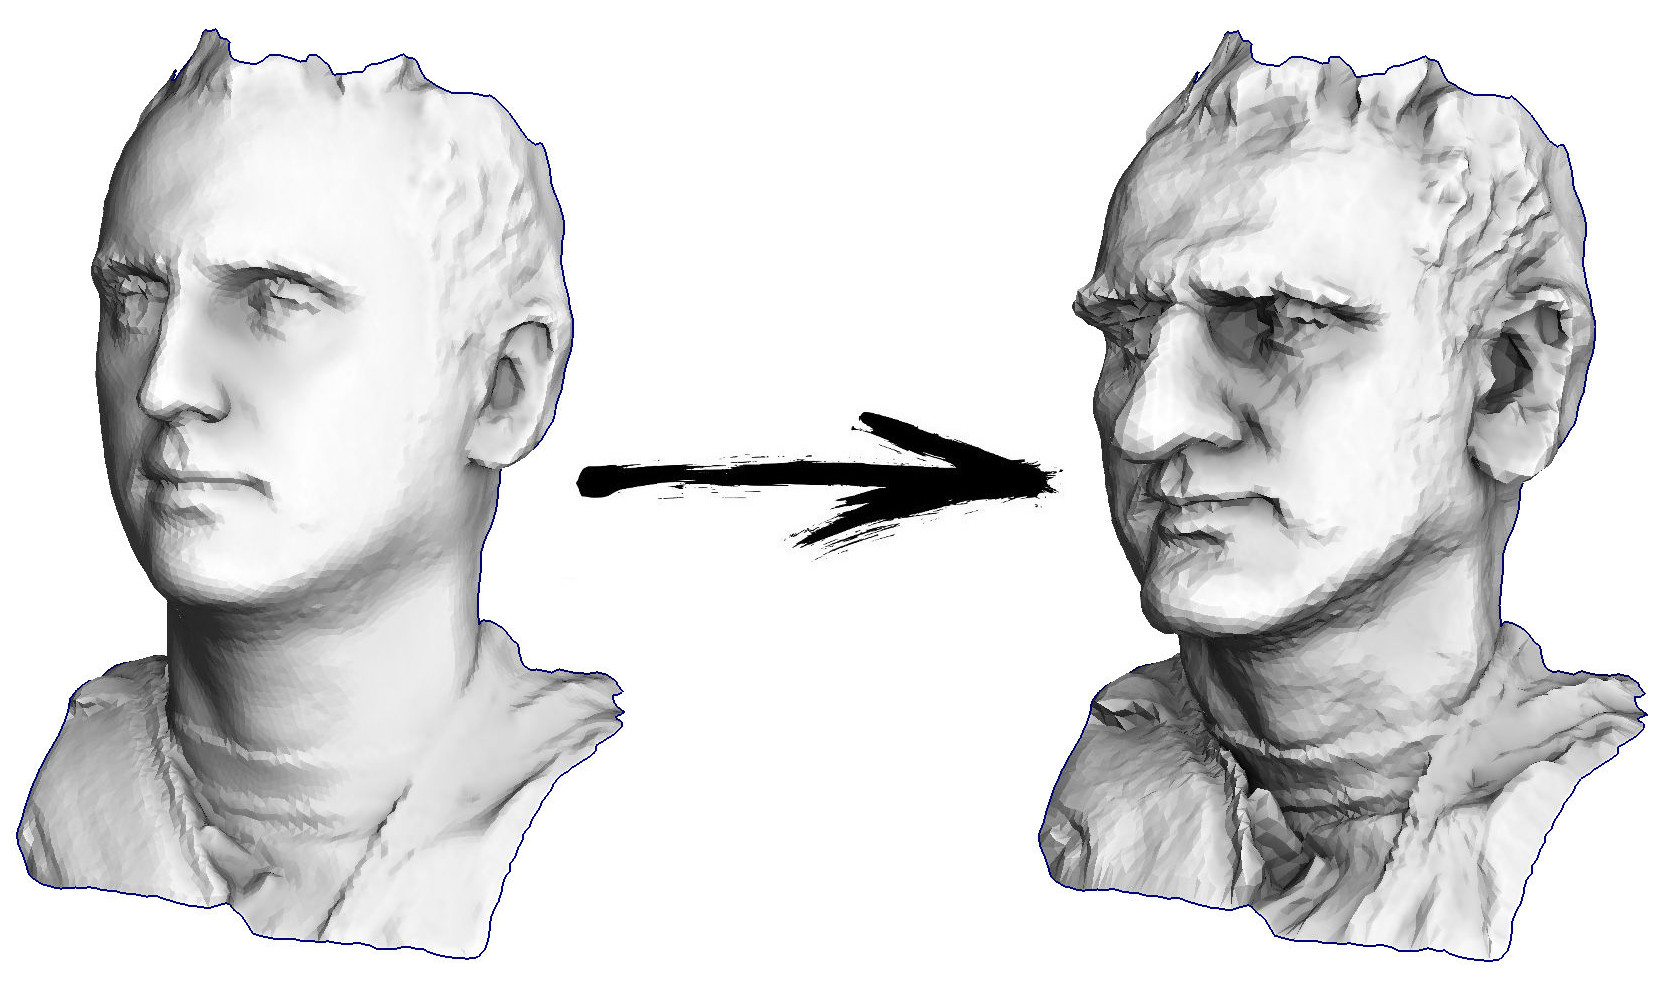
\includegraphics[width=.8\linewidth]{caricature.jpg}
\end{center}

\chapter{Is probability theory well-founded or do you believe in the theory of evolution?}

This short section is not mandatory for the understanding of the main course; 
the idea behind is to warm up before attacking code and formulae.
I’ll start with the least squares methods through the maximum likelihood estimation;
this requires some (at least superficial) knowledge of probability theory. 
So, right from the beginning, I would like to digress a little.


\begin{wrapfigure}{r}{.2\linewidth}

\includegraphics[width=\linewidth]{stop-following-me.png}
\end{wrapfigure}
I was once asked if I believed in evolutionary theory. 
Take a short break, think about how you would answer.
Being puzzled by the question, I have answered that I find it plausible. 
Scientific theory has little to do with faith.
In short, a theory only builds a model of the world, and there is no need to believe in it.
Moreover, the Popperian criterion\cite{} requires a scientific theory be able to be falsifiable. 
A solid theory must possess, first of all, the power of prediction.
For example, if you genetically modify crops in such a way that they produce pesticides themselves, 
it is only logical that pesticide-resistant insects would appear. 
However, it is much less obvious that this process can be slowed down by growing regular plants side by side with genetically modified plants. 
Based on evolutionary theory, the corresponding modelling has made this prediction\cite{}, and it seems to have been validated\cite{}.

\paragraph*{Wait, what is the connection?}

As I mentioned earlier, the idea is to approach the least squares through the principle of maximum likelihood. 
Let us illustrate by example. 
Suppose we are interested in penguins body height, but we are only able to measure a few of these magestic birds.
It is reasonable to introduce the body height distribution model into the task; most often it is supposed to be normal.
A normal distribution is characterized by two parameters: the average value and the standard deviation.
For each fixed value of parameters, we can calculate the probability that the measurements we made would be generated.
Then, by varying the parameters, we will find those that maximize the probability.

Thus, to work with maximum likelihood we need to operate in the notions of probability theory.
We will informally define the concept of probability and plausibility,
but I would like to focus on another aspect first.
I find it surprisingly rare to see people paying attention to the word \textit{theory} in ``probability theory''.

What are the origins, values and scope of probabilistic estimates? 
For example, Bruno de Finetti said that the probability is nothing but a subjective analysis of the probability that something will happen, 
and that this probability does not exist out of mind. 
It's a person's willingness to bet on something to happen. 
This opinion is directly opposed to the view of people adhering to the classical/frequentist interpretation of probabilty.
They assume that the same event can be repeated many times, and the ``probability'' of a particular result is associated with 
the frequency of a particular outcome during repeated well-defined random experiment trials.
In addition to subjectivists and frequentists, there are also objectivists who argue that probabilities are real aspects of the universe, 
and not a mere measurement of the observer's degree of confidence.

In any case, all three scientific schools in practice use the same apparatus based on Kolmogorov's axioms.
Let us provide an indirect argument, from a subjectivistic point of view, in favor of the probability theory based on Kolmogorov's axioms.
We will list the axioms later, first assume that we have a bookmaker who takes bets on the next World Cup. 
Let us have two events: $a=$ Uruguay will be the champion, $b=$ Germany wins the cup.
The bookmaker estimates the chances of the Uruguayan team to win at 40\%, and the chances of the German team at 30\%.
Clearly, both Germany and Uruguay cannot win at the same time, so the chance of $a\wedge b$ is zero. 
At the same time, the bookmaker thinks that the probability that either Uruguay or Germany (and not Argentina or Australia) will win is 80\%.
Let's write it down in the following form:
$$P(a) = .4  \qquad  P(a\wedge b) = 0 \qquad P(b) = .3 \qquad P(a\vee b) = .8$$
	
If the bookmaker asserts that his degree of confidence in the event $a$ is equal to 0.4, i.e., $P(a) = 0.4$, 
then the player can choose whether he will bet on or against the statement $a$,
placing amounts that are compatible with the degree of confidence of the bookmaker.
It means that the player can make a bet on the event $a$, placing \$4 against \$6 of the bookmaker's money.
Or the player can bet \$6 on the event $\neg a$ against \$4 of bookmaker's money.

If the bookmaker's confidence level does not accurately reflect the state of the world, 
we can expect that in the long run he will lose money to players whose beliefs are more accurate.
However, it is very curious that in this particular example, the player has a winning strategy: he can make the bookmaker lose money for \textit{any} outcome.
Let us illustrate it:

\vspace{2mm}
\begin{tabular}{cccccc}
	\multicolumn{2}{c}{Player's bets}  &  \multicolumn{4}{c}{Result for the bookmaker} \\
	\hline
	{\tiny Bet event} & {\tiny Bet amount} & {\tiny $a\wedge b$} & {\tiny $a\wedge \neg b$} &  {\tiny $\neg a\wedge b$} &  {\tiny $\neg a\wedge\neg b$} \\
	\hline
	$a$             & 4-6 & -6 & -6 &  4 &  4 \\
	$b$             & 3-7 & -7 &  3 & -7 &  3 \\
	$\neg(a\vee b)$ & 2-8 &  2 &  2 &  2 & -8 \\
	\hline
	&     &-11 & -1 & -1 & -1
\end{tabular}
\vspace{2mm}

The player makes three bets, and independently of the outcome, he always wins. 
Please note that in this case we do not even take into account whether Uruguay or Germany were favorits or outsiders, 
the loss of the bookmaker is guaranteed! 
This unfortunate (for the bookmaker) situation happened because he did not respect the third axiom of Kolmogorov, let us list all three of them:
\begin{itemize}
\item $0\leq P(a)\leq 1$: all probabilities range from 0 to 1.
\item $P(true)=1$, $P(false) = 0$: true statements have probability of 1 and false probability of 0.
\item $P(a\vee b) = P(a) + P(b) - P(a\wedge b)$: this one is also very intuitive.
All cases where the statement $a$ is true, together with those where $b$ is true,
cover all those cases where the statement $a\vee b$ is true; however the intersection $a\wedge b$ is counted twice in the sum, therefore it is necessary to subtract $P(a\wedge b)$.
\end{itemize}

Let us define the word ``event'' as ``a subset of the unit square''. 
Define the word ``probability of event'' as ``area of the corresponding subset''. 
Roughly speaking, we have a large dartboard, and we close our eyes and shoot at it. 
The chances that the dart hits a given region of the dartboard are directly proportional to the area of the region. 
A true event in this case is the entire square, and false events are those of zero measure, for example, any given point. 
Figure~\ref{fig:kolmogorov} illustrates the axioms.
\begin{figure}[htb!]
\centering
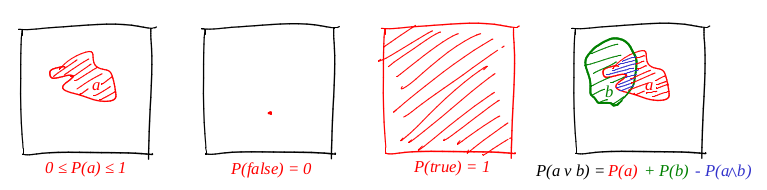
\includegraphics[width=.8\columnwidth]{axiomes.png}
\caption{A graphical illustration for the Kolmogorov's axioms}
\label{fig:kolmogorov}
\end{figure}

In 1931, de Finetti proved a very strong proposition:

\vspace{4mm}

\textit{If a bookmaker is guided by beliefs which break the axioms of the theory of probability,
then there exists such a combination of bets of the player which guarantees the loss for the bookmaker (a prize for the player) at each bet.
}

\vspace{4mm}

Probability axioms can be considered as the limiting set of probabilistic beliefs that some agent can adhere to.
Note that if a bookmaker respects Kolmogorov's axioms, it does not imply that he will win (leaving aside the fees),
however, if he does not respect the axioms, he is guaranteed to lose.
Other arguments have been put forward in favour of the probability theory;
but it is the practical success of probability-based reasoning systems that has proved to be very attractive.

To conclude the digression, it seems reasonable to base our reasoning on the probability theory.
Now let us proceed to maximum likelihood estimation, thus motivating the least squares.

\chapter{Maximum likelihood through examples}
\section{First example: coin toss}
Let us consider a simple example of coin flipping, also known as the Bernoulli's scheme. 
We conduct $n$ experiments, two events can happen in each one (``success'' or ``failure''): 
one happens with probability $p$, the other one with probability $1-p$. 
Our goal is to find the probability of getting exactly $k$ successes in these $n$ experiments. 
This probability is given by the Bernoulli's formula:
$$
P(k;n,p) = C_n^k p^k (1-p)^{n-k}
$$

Let us take an ordinary coin ($p=1/2$), flip it ten times ($n=10$), and count how many times we get the tails:
$$P(k) = C_{10}^k \frac{1}{2^k}\left(1-\frac{1}{2}\right)^{10-k} = \frac{C_{10}^k}{2^{10}}$$
Figure~\ref{fig:binomial}, left shows what a probability density graph looks like.

\begin{figure}[htb!]
\centering
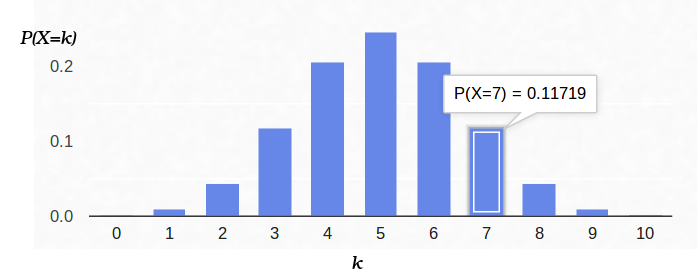
\includegraphics[width=.48\columnwidth]{binomial-05.png}
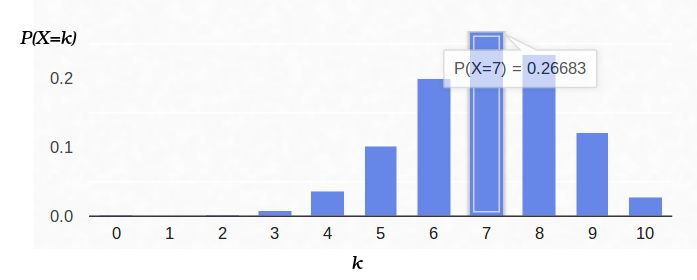
\includegraphics[width=.48\columnwidth]{binomial-07.png}
\caption{\textbf{Left:} probability density graph for the Bernoulli's scheme with $p=1/2$. \textbf{Right:} probability density graph for the Bernoulli's scheme with $p=7/10$.}
\label{fig:binomial}
\end{figure}

Thus, if we have fixed the probability of ``success'' ($1/2$) and also fixed the number of experiments (10), 
then the possible number of ``successes'' can be any integer between 0 and 10, but these outcomes are not equiprobable. 
It is clear that five ``successes'' are much more likely to happen than none. For example, the probability encountering seven tails is about 12\%.

Now let us look at the same problem from a different angle. 
Suppose we have a real coin, but we do not know its distribution of a priori probability of ``success''/``failure''. 
However, we can toss it ten times and count the number of ``successes''. 
For example, we have counted seven tails.
Would it help us to evaluate $p$?

We can try to fix $n=10$ and $k=7$ in the Bernoulli's formula, leaving $p$ as a free parameter:
$$\mathcal{L}(p) = C_{10}^7 p^7 (1-p)^3$$

Then the Bernoulli's formula can be interpreted as the plausibility of the parameter being evaluated (in this case $p$).
I have even changed the function notation, now it is denoted as $\mathcal L$ (likelihood).
That is being said, the likelihood is the probability to generate the observation data (7 tails out of 10 experiments) for the given value of the parameter(s).
For example, the likelihood of a balanced coin ($p=1/2$) with seven tails out of ten tosses is approximately 12\%. 
Figure~\ref{fig:likelihood} plots the likelihood function for the observation data with 7 tails out of 10 experiments.

\begin{figure}[htb!]
\centering
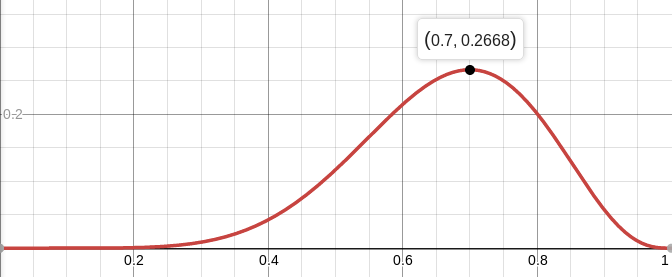
\includegraphics[width=.5\columnwidth]{likehood-07.png}
\caption{The plot of the likelihood function $\mathcal{L}(p)$ for the observation data with 7 tails out of 10 experiments.}
\label{fig:likelihood}
\end{figure}

So, we are looking for the parameter value that maximizes the likelihood of producing the observations we have.
In our particular case, we have a function of one variable, and we are looking for its maximum.
In order to make things easier, I will not search for the maximum of $\mathcal L$, but for the maximum of $\log \mathcal L$.
The logarithm is a strictly monotonous function, so maximizing both is equivalent.
The logarithm has a nice property of breaking down products into sums that are much more convenient to differentiate.
So, we are looking for the maximum of this function:
$$\log \mathcal{L}(p) = \log C_{10}^7 + 7 \log p + 3\log (1-p)$$

That's why we equate it's derivative to zero:
$$\frac{d \log \mathcal{L}}{dp} = 0$$

The derivative of $\log x = \frac{1}{x}$, therefore:
$$\frac{d \log \mathcal{L}}{dp} = \frac{7}{p} - \frac{3}{1-p} = 0$$

That is, the maximum likelihood (about 27\%) is reached at the point $p=7/10$.
Just in case, let us check the second derivative:
$$\frac{d^2 \log \mathcal{L}}{dp^2} = -\frac{7}{p^2} - \frac{3}{(1-p)^2}$$

In the point $p=7/10$ it is negative, therefore this point is indeed a maximum of the function $\mathcal{L}$:
$$\frac{d^2 \log \mathcal{L}}{dp^2}(0.7)  \approx -48 < 0$$

Figure~\ref{fig:binomial} shows the probability density graph for the Bernoulli's scheme with $p=7/10$.


\section{Second example: analog-to-digital converter (ADC)}

Let us imagine that we have a constant physical quantity that we want to measure; for example, it can be a length to measure with a ruler or a voltage with a voltmeter.
In the real world, any measurement gives \textit{an approximation} of this value, but not the value itself.
The methods I am describing here were developed by Gauss at the end of the 18th century, when he measured the orbits of celestial bodies
\footnote{Note that Legendre has published an equivalent method in 1805, 
whereas Gauss' first publication is dated by 1809. Gauss has always claimed that he had been using the method since 1795,
and this is a very famous priority dispute~\cite{https://projecteuclid.org/download/pdf_1/euclid.aos/1176345451} in the history of statistics.
There are, however, numerous evidence to support the thesis that Gauss possessed the method before Legendre, but he was late in his communication.}.
~\cite{Theoria Motus Corporum Coelestium}

For example, if we measure the battery voltage $N$ times, we get $N$ different measurements. Which of them should we take? All of them! 
So, let us say that we have $N$ measurements $U_j$:
$$
\{U_j\}_{j=1}^{N}
$$

Let us suppose that each measurement $U_j$ is equal to the real value plus the Gaussian noise. 
The noise is characterized by two parameters --- the center of the Gaussian bell and its ``width''. 
In this case, the probability density can be expressed as follows:
$$
p(U_j) = \frac{1}{\sqrt{2\pi}\sigma} \exp\left(-\frac{(U_j-U)^2}{2\sigma^2}\right)
$$

That is, having $N$ measurements $U_j$, our goal is to find the parameters $U$ and $\sigma$ that maximize the likelihood.
The likelihood (I have already applied the logarithm) can be written as follows:
\begin{align*}
\log \mathcal{L}(U,\sigma) & = \log \left(\prod\limits_{j=1}^N  \frac{1}{\sqrt{2\pi}\sigma} \exp\left(-\frac{(U_j-U)^2}{2\sigma^2}\right)\right) =\\
& = \sum\limits_{j=1}^N \log \left(\frac{1}{\sqrt{2\pi}\sigma} \exp\left(-\frac{(U_j-U)^2}{2\sigma^2}\right)\right) = \\
& = \sum\limits_{j=1}^N \left(\log \left(\frac{1}{\sqrt{2\pi}\sigma}\right) -\frac{(U_j-U)^2}{2\sigma^2}\right) = \\
& = -N \left(\log\sqrt{2\pi} + \log\sigma\right) - \frac{1}{2\sigma^2} \sum\limits_{j=1}^N (U_j-U)^2
\end{align*}

And then everything is strictly as it used to be, we equate the partial derivatives to zero:
$$
\frac{\partial\log\mathcal{L}}{\partial U}    =  \frac{1}{\sigma^2}\sum\limits_{j=1}^N (U_j-U) = 0 
$$

The most plausible estimation of the unknown value $U$ is the simple average of all measurements:
$$
U = \frac{\sum\limits_{j=1}^N U_j}{N}
$$

And the most plausible estimation of $\sigma$ turns out to be the standard deviation:
$$
\frac{\partial\log\mathcal{L}}{\partial\sigma} =  -\frac{N}{\sigma} + \frac{1}{\sigma^3}\sum\limits_{j=1}^N (U_j-U)^2 = 0
$$

$$
\sigma = \sqrt{\frac{\sum\limits_{j=1}^N (U_j-U)^2}{N}} 
$$

Such a convoluted way to obtain a simple average of all measurements\dots
In my humble opinion, the result is worth the effort.
By the way, averaging multiple measurements of a constant value in order to increase the accuracy of measurements is quite a standard practice.
For example, ADC averaging. Note that the hypothesis of Gaussian noise is not necessary in this case, it is enough to have an unbiased noise.


\section{Third exampe, still 1D}

Let us re-consider the previous example with a small modification.
Let us say that we want to measure the resistance of a resistor.
We have a bench top power supply with current regulation.
That is, we control the current flowing through the resistance and we can measure the voltage required for this current.
So, our ``ohmmeter'' evaluates the resistance through $N$ meausrements $U_j$ for each reference current $I_j$:
$$
\{I_j, U_j\}_{j=1}^{N}
$$

If we draw these points on a chart (Figure~\ref{fig:URI}), the Ohm's law tells us that we are looking for the slope of the blue line that approximates the measurements.
\begin{figure}[htb!]
\centering
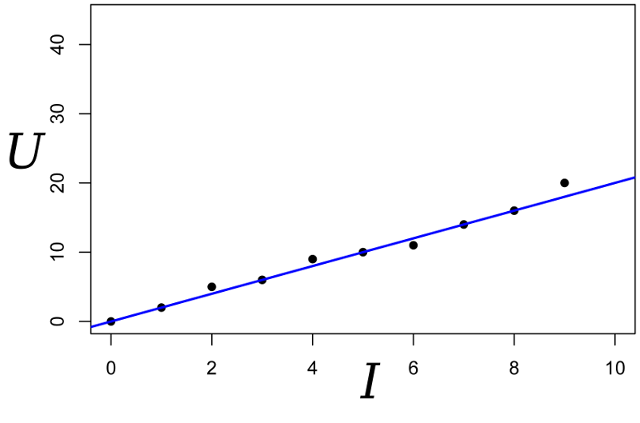
\includegraphics[width=.5\columnwidth]{URI.png}
\caption{Having $N$ meausrements $U_j$ for each reference current $I_j$, we are looking for the slope of the blue line that approximates the measurements through the Ohm's law.}
\label{fig:URI}
\end{figure}


Let us write the expression of the (logarithm of) likelihood of the parameters:
\begin{align*}
\log \mathcal{L}(R,\sigma) & = \log \left(\prod\limits_{j=1}^N  \frac{1}{\sqrt{2\pi}\sigma} \exp\left(-\frac{(U_j-R I_j)^2}{2\sigma^2}\right)\right) =\\
& = -N \left(\log\sqrt{2\pi} + \log\sigma\right) - \frac{1}{2\sigma^2} \sum\limits_{j=1}^N (U_j- R I_j)^2
\end{align*}

As usual, we equate the partial derivatives to zero:
\begin{align*}
\frac{\partial\log\mathcal{L}}{\partial R} &=  -\frac{1}{2\sigma^2}\sum\limits_{j=1}^N -2I_j (U_j- R I_j) = \\
&= \frac{1}{\sigma^2}\left(\sum\limits_{j=1}^N I_jU_j - R\sum\limits_{j=1}^N I_j^2\right) = 0
\end{align*}

Then the most plausible resistance $R$ can be found with the following formula:
$$
R = \frac{\sum\limits_{j=1}^N I_jU_j}{\sum\limits_{j=1}^N I_j^2}
$$

This result is somewhat less obvious than the simple average of all measurements in the previous example.
Note that if we take one hundred measurements with $\approx 1A$ reference current and one measurement with $\approx 1kA$ reference current,
then the first hundred measurements would barely affect the result. Let's remember this fact, we will need it later.

\section{Fourth example: back to the least squares}
You have probably already noticed that in the last two examples, maximizing the logarithm of the likelihood is equivalent to minimizing the sum of squared estimation errors.
Let us consider one more example.
Say we want to calibrate a spring scale with a help of reference weights.
Suppose we have $N$ reference weights of mass $x_j$; we weigh them with the scale and measure the length of the spring.
So, we have $N$ spring lengths $y_j$:
$$
\{x_j, y_j\}_{j=1}^{N}
$$

Hooke's law tells us that spring stretches linearly on the force applied;
this force includes the reference weight and the weight of the spring itself. 
Let us denote the spring stiffness as $a$, and the spring length streched under under its own weight as $b$. 
Then we can express the plausibility of our measurements (still under the Gaussian measurement noise hypothesis) in this way:
\begin{align*}
\log \mathcal{L}(a, b,\sigma) & = \log \left(\prod\limits_{j=1}^N  \frac{1}{\sqrt{2\pi}\sigma} \exp\left(-\frac{(y_j - a x_j - b)^2}{2\sigma^2}\right)\right) =\\
& = -N \left(\log\sqrt{2\pi} + \log\sigma\right) - \frac{1}{2\sigma^2} \sum\limits_{j=1}^N (y_j- a x_j - b)^2
\end{align*}

Maximizing the likelihood of $\mathcal L$ is equivalent to minimizing the sum of the squared estimation error, i.e., we are looking for the minimum of the function $S$ defined as follows:
$$
S(a, b) = \sum\limits_{j=1}^N (y_j- a x_j - b)^2
$$


\begin{figure}[htb!]
\centering
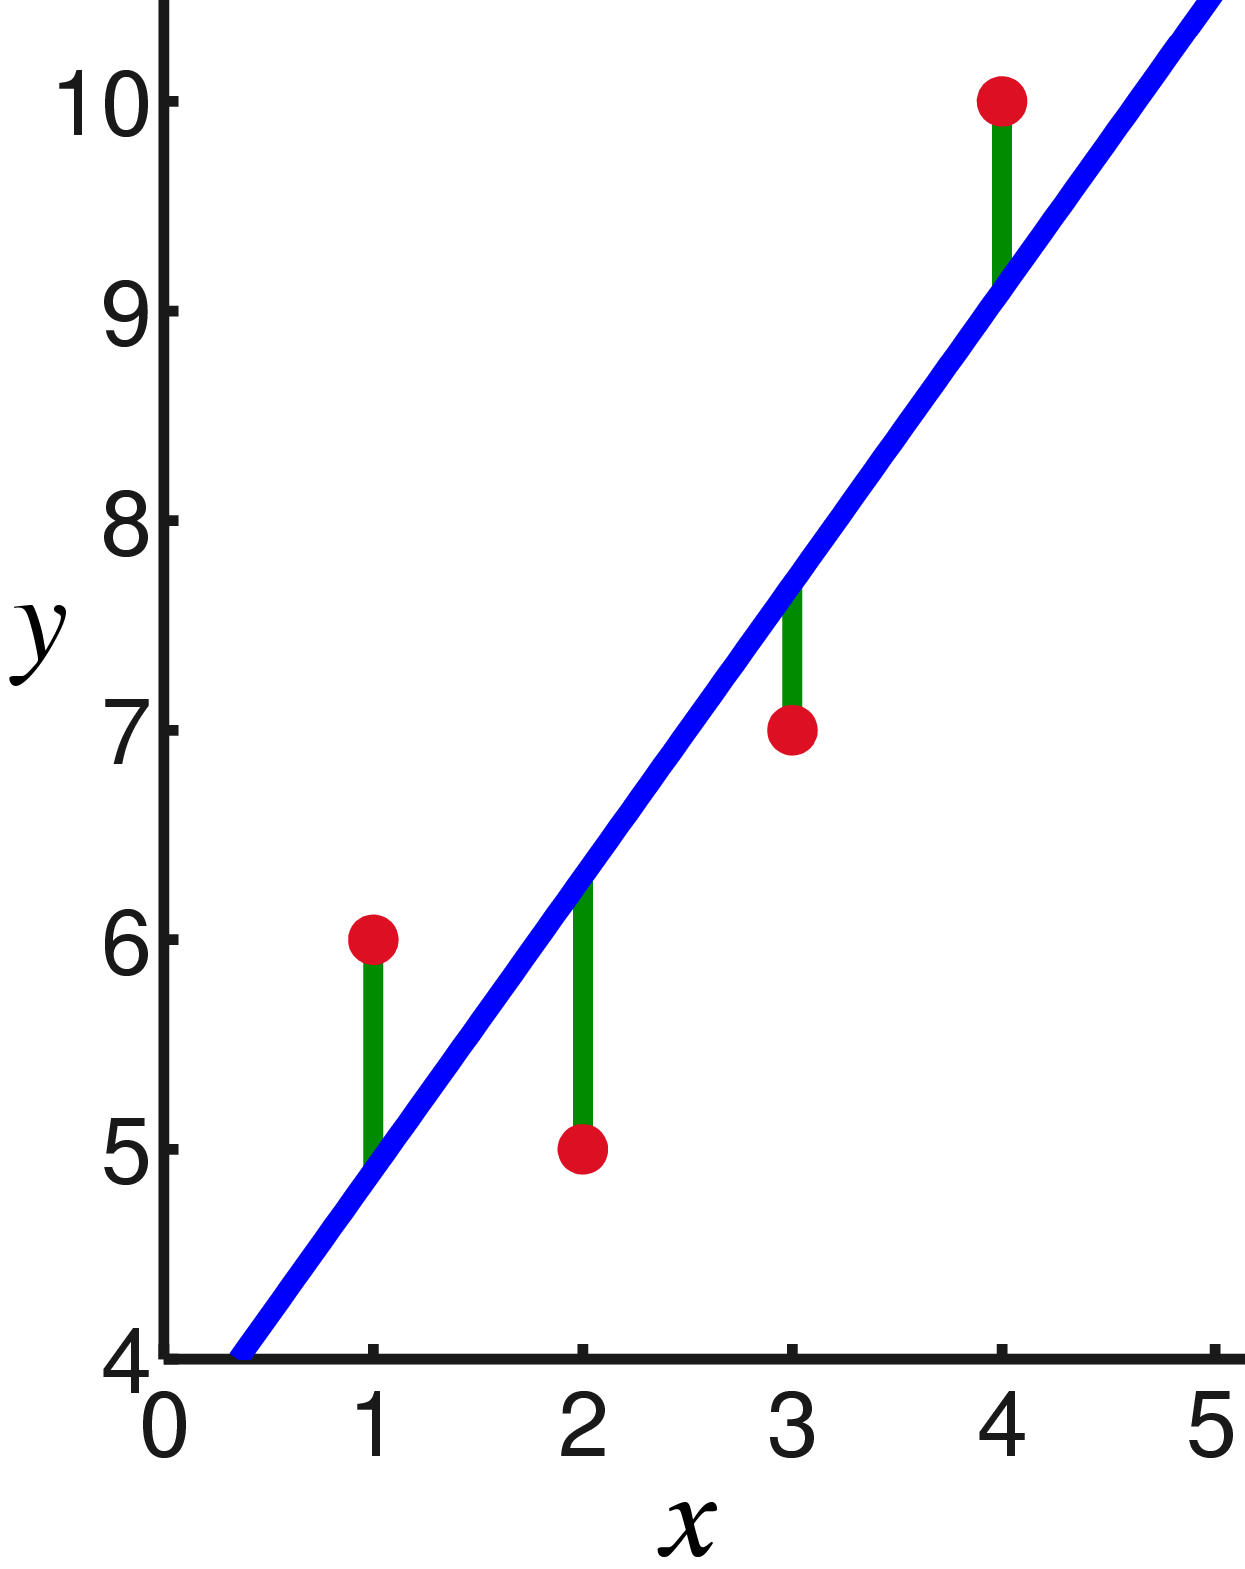
\includegraphics[width=.2\columnwidth]{c5aa80f6a2e9575abfa7b3dfdabf5c5a.png}
\caption{To calibrate the spring scale, we can solve the linear regression problem.}
\label{fig:regression}
\end{figure}

Figure~\ref{fig:regression} illustrates the formula: we are looking for such a straight line that minimizes the sum of squared lengths of green segments.
And then the derivation is quite straightforward:
\begin{align*}
\frac{\partial S}{\partial a} &= \sum\limits_{j=1}^N 2 x_j (a x_j + b - y_j) = 0 \\
\frac{\partial S}{\partial b} &= \sum\limits_{j=1}^N 2 (a x_j + b - y_j) = 0
\end{align*}

We obtain a system of two linear equations with two unknowns:
$$
\left \{ \begin{array}{r l}
a \sum\limits_{j=1}^N x_j^2 + b \sum\limits_{j=1}^N x_j  & = \sum\limits_{j=1}^N x_j y_j\\
a \sum\limits_{j=1}^N x_j   + b N                        & = \sum\limits_{j=1}^N y_j
\end{array} \right.
$$

Use your favorite method to obtain the following solution:
\begin{align*}
a &= \frac{N \sum\limits_{j=1}^N x_j y_j - \sum\limits_{j=1}^N x_j \sum\limits_{j=1}^N y_j}{N\sum\limits_{j=1}^N x_j^2 - \left(\sum\limits_{j=1}^N x_j\right)^2} \\
b &= \frac{1}{N}\left(  \sum\limits_{j=1}^N y_j - a  \sum\limits_{j=1}^N x_j \right)
\end{align*}

\section*{Conclusion}
The least squares method is a particular case of maximizing likelihood in cases where the probability density is Gaussian.
If the density is not Gaussian, the least squares approach can produce an estimate different from the MLE (maximum likelihood estimation).
By the way, Gauss conjectured that the type of noise is of no importance, and the only thing that matters is the independence of trials.

As you have already noticed, the more we parameters we have, the more cumbersome the analytical solutions are.
Fortunately, we are not living in XVIII century anymore, we have computers!
Next we will try to build a geometric intuition on least squares, and see how can least squares problems be efficiently implemented.


\chapter{Introduction to systems of linear equations}

\section{Smooth an array}
\label{sec:arraysmooth}
The time has come to write some code. Let us examine the following program:
\inputminted[frame=single,linenos=true]{python}{listings/example_3.1.py}

Top left image of the Figure~\ref{fig:linsys_smooth} shows the initialization of the array \mintinline{python}{x}.

\begin{figure}[ht]
    \centering
    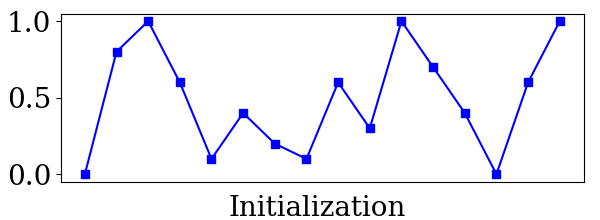
\includegraphics[width=.32\linewidth]{example_3.1_0.png}
    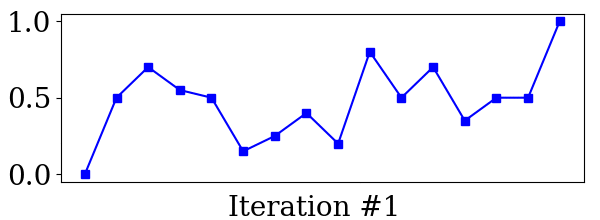
\includegraphics[width=.32\linewidth]{example_3.1_1.png}
    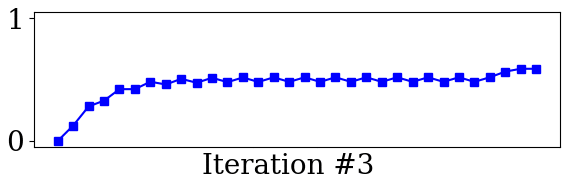
\includegraphics[width=.32\linewidth]{example_3.1_2.png}
    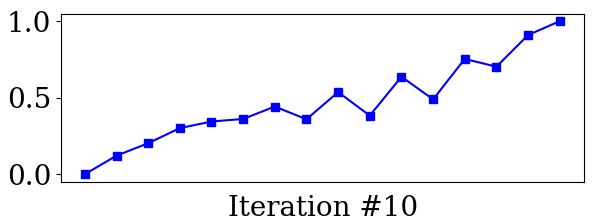
\includegraphics[width=.32\linewidth]{example_3.1_3.png}
    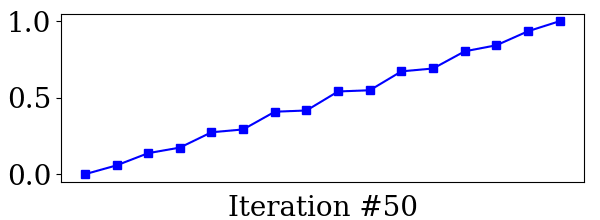
\includegraphics[width=.32\linewidth]{example_3.1_4.png}
    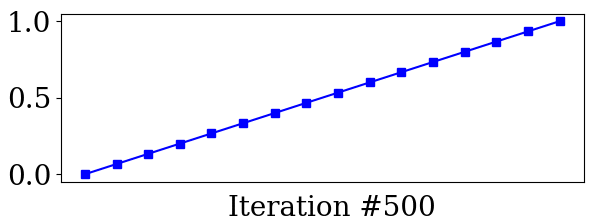
\includegraphics[width=.32\linewidth]{example_3.1_5.png}
\caption{Smoothing an array: first 500 iterations of the program from \S~\ref{sec:arraysmooth}.}
    \label{fig:linsys_smooth}
\end{figure}



\section{The Jacobi and Gauss-Seidel iterative methods}
\label{sec:gauss-seidel}
$$
\left\{
\begin{array}{cccccccc}
a_{11}x_1 & + &  a_{12}x_2  &+      & \cdots & + & a_{1n}x_n &= b_1\\
a_{21}x_1 & + &  a_{22}x_2  &+      & \cdots & + & a_{2n}x_n &= b_2\\
          &   &             &\vdots &        &   &           &     \\
a_{n1}x_1 & + &  a_{n2}x_2  &+      & \cdots & + & a_{nn}x_n &= b_n\\
\end{array}
\right.
$$

\begin{align*}
x_1 &= \frac{1}{a_{11}}(b_1 - a_{12}x_2 - a_{13}x_3 - \cdots - a_{1n}x_n)\\
x_2 &= \frac{1}{a_{22}}(b_2 - a_{21}x_1 - a_{23}x_3 - \cdots - a_{2n}x_n)\\
    & \qquad \vdots \\
x_n &= \frac{1}{a_{nn}}(b_n - a_{n1}x_1 - a_{n2}x_2 - \cdots - a_{n,n-1}x_{n-1})
\end{align*}

$$\vec{x}^{(0)}=\left(x_1^{(0)}, x_2^{(0)}, \dots, x_n^{(0)}\right)$$

$$\vec{x}^{(1)}=\left(x_1^{(1)}, x_2^{(1)}, \dots, x_n^{(1)}\right)$$

\begin{align*}
x_1^{(1)} &= \frac{1}{a_{11}}(b_1 - a_{12}x_2^{(0)} - a_{13}x_3^{(0)} - \cdots - a_{1n}x_n^{(0)})\\
x_2^{(1)} &= \frac{1}{a_{22}}(b_2 - a_{21}x_1^{(0)} - a_{23}x_3^{(0)} - \cdots - a_{2n}x_n^{(0)})\\
    & \qquad \vdots \\                                                                          
x_n^{(1)} &= \frac{1}{a_{nn}}(b_n - a_{n1}x_1^{(0)} - a_{n2}x_2^{(0)} - \cdots - a_{n,n-1}x_{n-1}^{(0)})
\end{align*}

$$\vec{x}^{(k)}=\left(x_1^{(k)}, x_2^{(k)}, \dots, x_n^{(k)}\right)$$

$$
x_i^{(k)} = \frac{1}{a_{ii}} \left(b_i - \sum\limits_{j=1,j\neq i}^n a_{ij}x_j^{(k-1)} \right), \quad \text{for } i=1,2,\dots,n
$$

\begin{equation}
\label{eq:1d:smooth}
\left\{
\begin{array}{rl}
 x_0 &= 0 \\
x_1-x_0 &= x_2-x_1 \\
x_2-x_1 &= x_3-x_1 \\
     &  \vdots \\
x_{13}-x_{12}     &= x_{14}-x_{13} \\
x_{14}-x_{13}     &= x_{15}-x_{14} \\
x_{15} &= 1 \\
\end{array}
\right.
\end{equation}




$$
x_i^{(k)} = \frac{1}{a_{ii}} \left(b_i - \sum\limits_{j=1}^{i-1} a_{ij}x_j^{(k)} -  \sum\limits_{j=i+1}^n a_{ij}x_j^{(k-1)} \right), \quad \text{for } i=1,2,\dots,n
$$

\inputminted[frame=single,linenos=true]{python}{listings/example_3.2.py}


\begin{figure}[ht]
    \centering
    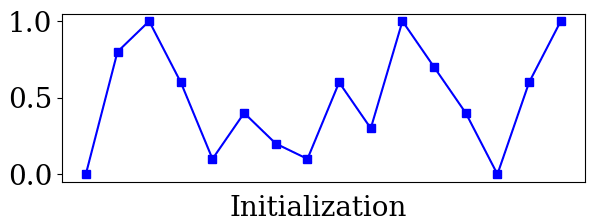
\includegraphics[width=.32\linewidth]{example_3.2_0.png}
    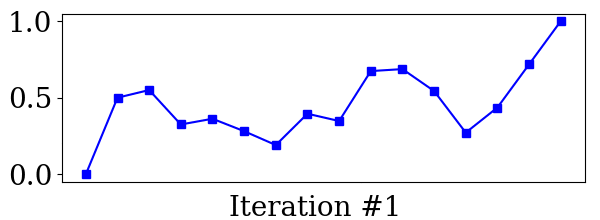
\includegraphics[width=.32\linewidth]{example_3.2_1.png}
    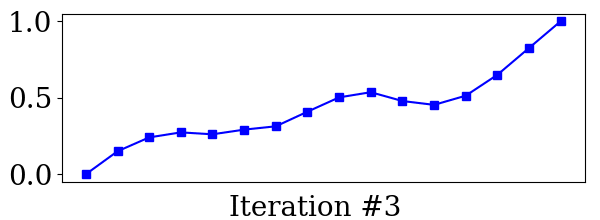
\includegraphics[width=.32\linewidth]{example_3.2_2.png}
    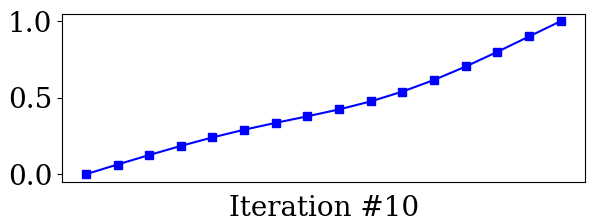
\includegraphics[width=.32\linewidth]{example_3.2_3.png}
    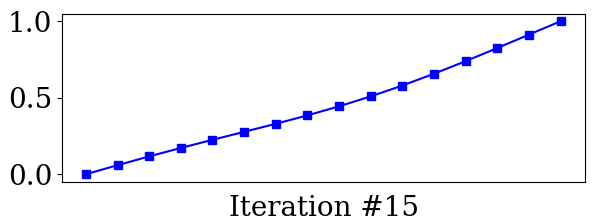
\includegraphics[width=.32\linewidth]{example_3.2_4.png}
    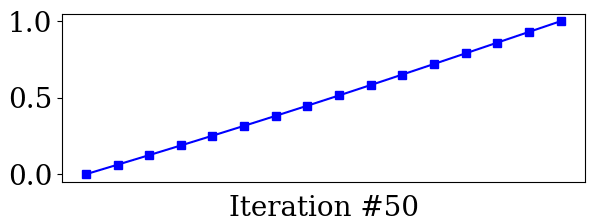
\includegraphics[width=.32\linewidth]{example_3.2_5.png}
    \caption{Linear function via Gauss-Seidel iteration (\S\ref{sec:gauss-seidel}).}
    \label{fig:linsys_smooth_constrain}
\end{figure}



\section{Prescribe the right hand side}
\label{sec:rhs}


\begin{equation}
%\label{eq:1d:smooth}
\nonumber
\left\{
\begin{array}{cccccccccccl}
 x_0 &       &       &       &      &        &         &          &          &          &         &= 0 \\
-x_0 & +2x_1 & -x_2  &       &      &        &         &          &          &          &         &= 0 \\
     & -x_1  & +2x_2 & -x_3  &      &        &         &          &          &          &         &= 0 \\
     &       & -x_2  & +2x_3 & -x_4 &        &         &          &          &          &         &= 0 \\
     &       &       &       &      & \ddots &         &          &          &          &         &  \vdots \\
     &       &       &       &      &        & -x_{11} & +2x_{12} & -x_{13}  &          &         &= 0 \\
     &       &       &       &      &        &         & -x_{12}  & +2x_{13} & -x_{14}  &         &= 0 \\
     &       &       &       &      &        &         &          & -x_{13}  & +2x_{14} & -x_{15} &= 0 \\
     &       &       &       &      &        &         &          &          &          &  x_{15} &= 1 \\
\end{array}
\right.
\end{equation}




\inputminted[frame=single,linenos=true]{python}{listings/example_3.3.py}
\begin{figure}[ht]
    \centering
    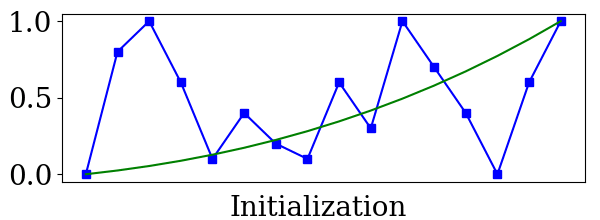
\includegraphics[width=.32\linewidth]{example_3.3_0.png}
    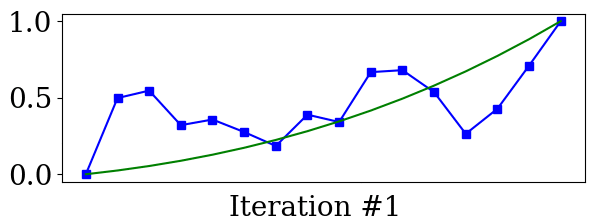
\includegraphics[width=.32\linewidth]{example_3.3_1.png}
    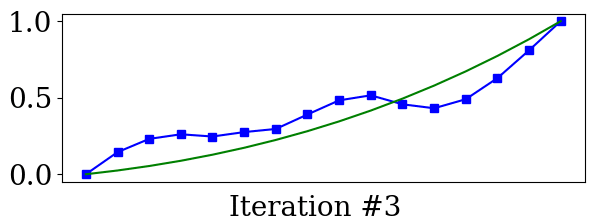
\includegraphics[width=.32\linewidth]{example_3.3_2.png}
    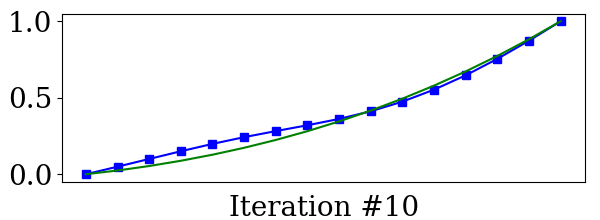
\includegraphics[width=.32\linewidth]{example_3.3_3.png}
    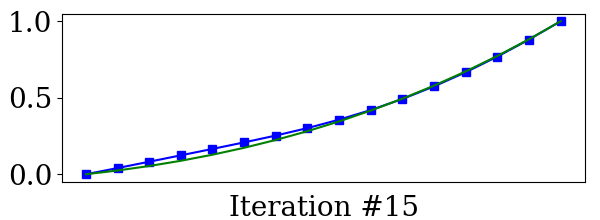
\includegraphics[width=.32\linewidth]{example_3.3_4.png}
    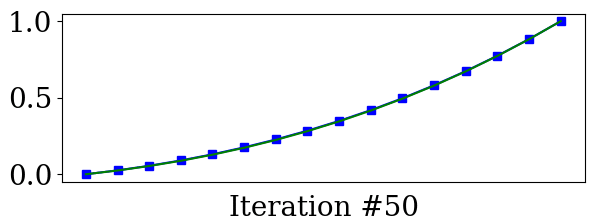
\includegraphics[width=.32\linewidth]{example_3.3_5.png}
    \caption{Reconstructing a cubic function (\S\ref{sec:rhs}); the ground truth is shown in green.}
    \label{fig:linsys_smooth_constrain}
\end{figure}


%\section{3D example}
%\begin{figure}[ht]
%	\centering
%	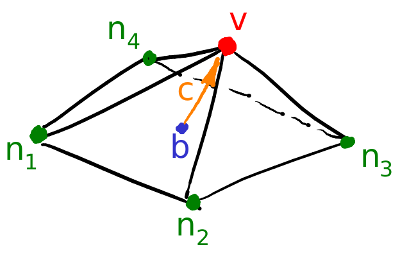
\includegraphics[width=.3\linewidth]{barycenter/1ring.png}
%	\caption{.}
%	\label{fig:????}
%\end{figure}

%\begin{figure}[ht]
%	\centering
%	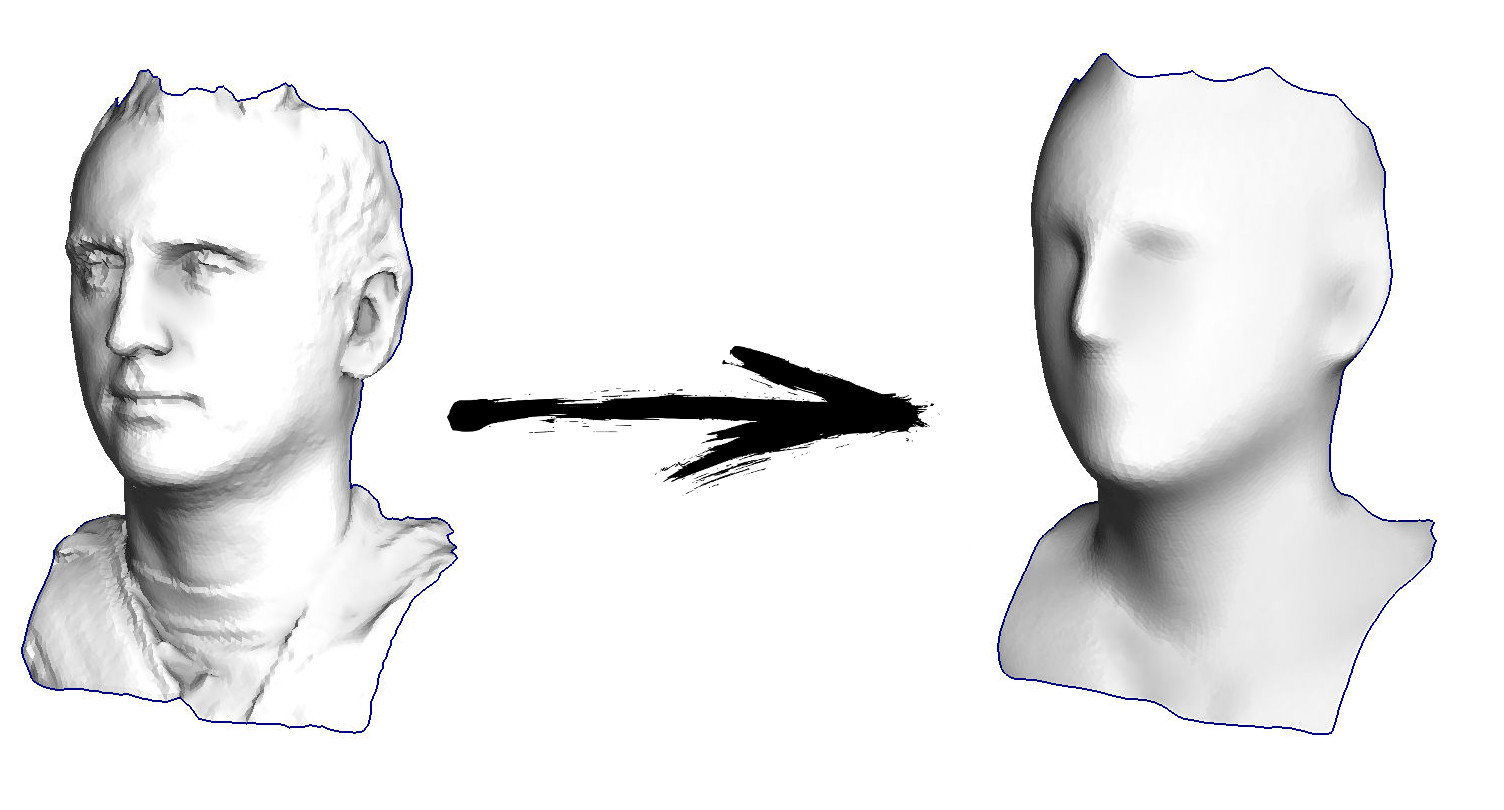
\includegraphics[width=.8\linewidth]{barycenter/ls-teaser2.jpg}
%	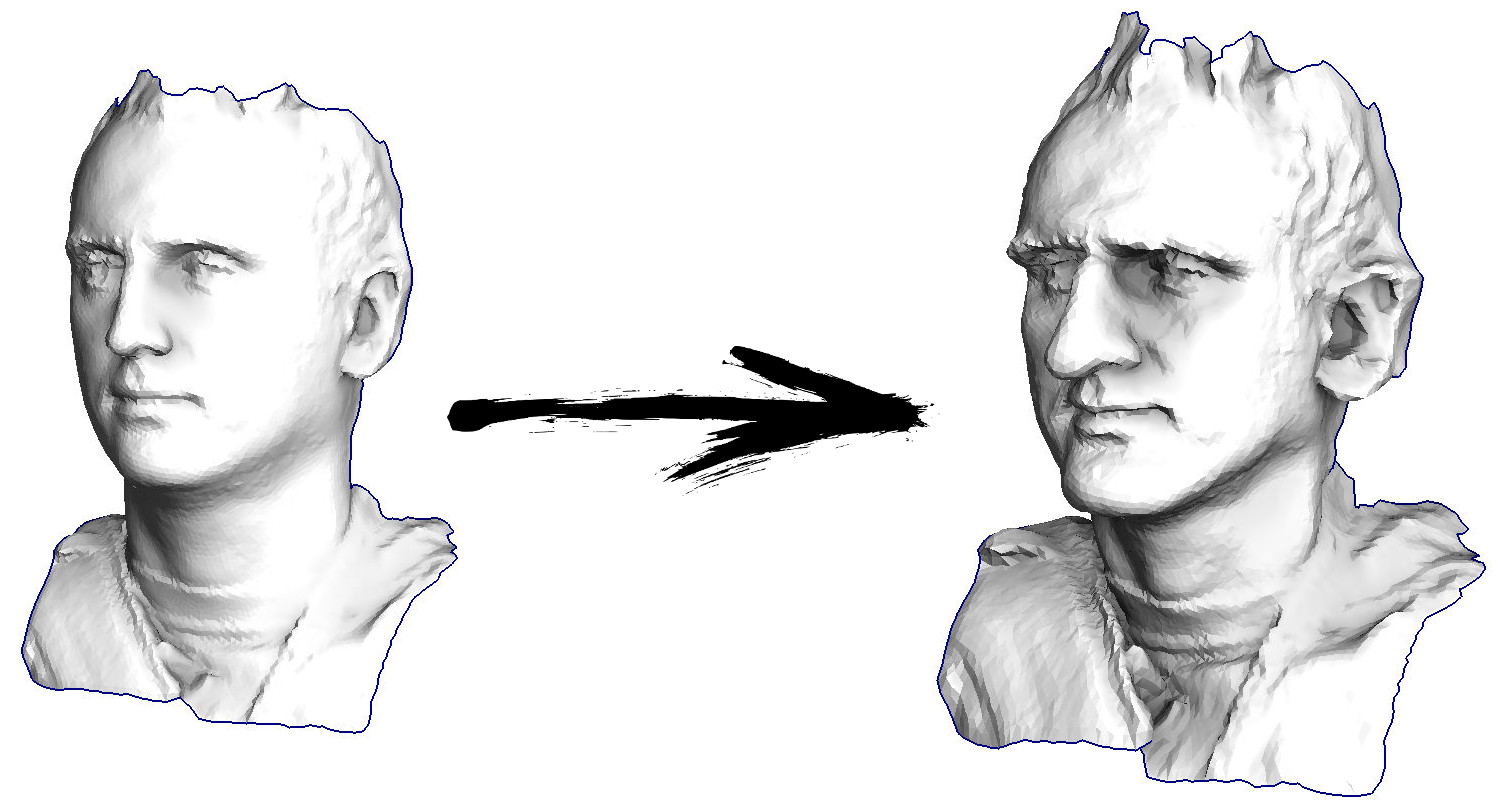
\includegraphics[width=.8\linewidth]{barycenter/ls-teaser.jpg}
%%	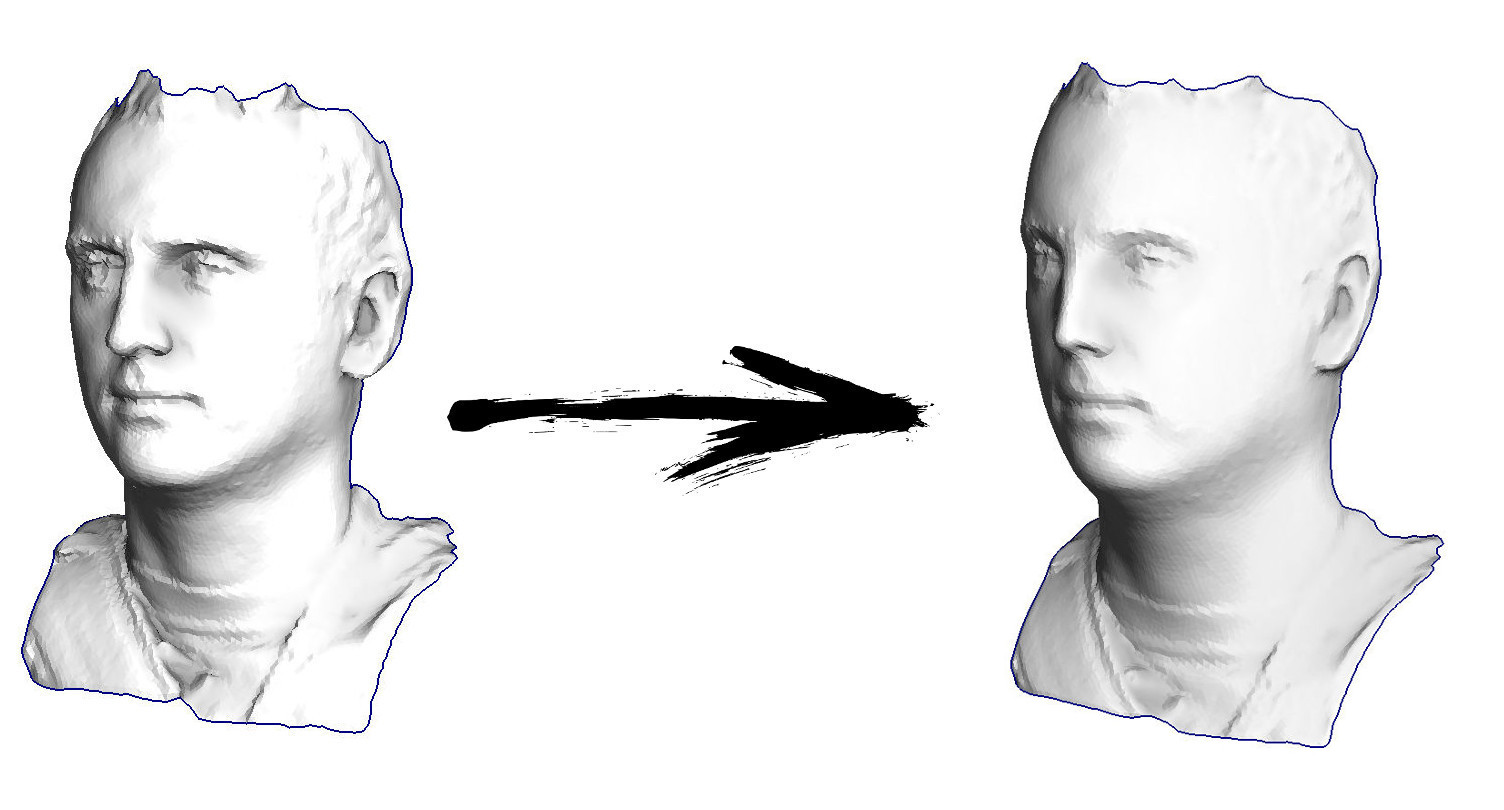
\includegraphics[width=.8\linewidth]{barycenter/ls-teaser3.jpg}
%	\caption{.}
%	\label{fig:????}
%\end{figure}


\chapter{Finite elements example: the Galerkin weighted residual method}

\section{Approximation of vectors}

\begin{figure}[ht]
	\centering
	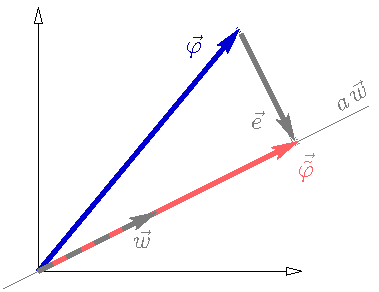
\includegraphics[width=.3\linewidth]{vector_approximation.pdf}
	\caption{.}
	\label{fig:vector_approximation}
\end{figure}


\section{Approximation of functions}

In this section we will consider a simple boundary value problem and its relation to systems of linear equations.
The boundary value problem is the problem of finding a solution to a given differential equation satisfying boundary conditions at the the boundary of a region.
Let us start with a ground truth function defined as 
$$
\varphi(x) := \frac{1}{6} x^3 + \frac{1}{2} x^2 + \frac{1}{3} x.
$$
This function is unknown, and we list it here to compare our solution to the ground truth.
Let us define a function $f(x) := x+1$.
It is simply the second derivative of $\varphi(x)$, but remember that $\varphi(x)$ is not known!
So, the problem is to find a function $\varphi(x)$ with prescribed second derivative and constrained at the limits of a region.
One possible instance of the boundary value problem can be written as follows:
$$
\left\{
\begin{split}
\frac{d^2}{dx^2}\varphi(x) = f(x), \quad 0 < x < 1\\
\varphi(0)=0, \quad \varphi(1)=1
\end{split}
\right.
$$
Here $f(x)$ is known, $\varphi(x)$ is unknown, but we have specified its values at the boundary.

In general, finite elements method searches for an \textit{approximated} solution of the problem.
Let us split the interval in $n$ parts, these subsegments are the \textit{elements}.
For example, for $n=3$ we can define four equispaced nodes $x_i$:
$$
x_0 := 0, \quad x_1 := \frac{1}{3}, \quad x_2 := \frac{2}{3}, \quad x_3 := 1.
$$
Note that equal distance is chosen here for the simplicity of presentation, and is not a requirement for the method.
Then a set of functions is to be defined over the elements; the approximated solution $\tilde{\varphi}$ is defined as a weighted sum of these functions.

For example, let us choose a set of piecewise linear functions (refer to Figure~\ref{fig:fem:blending} for an illustration):
$$
w_i(x) := \left\{
\begin{split}
\frac{x-x_{i-1}}{x_i-x_{i-1}}, & \quad x_{i-1}\leq x \leq x_i \\
\frac{x_{i+1}-x}{x_{i+1}-x_i}, & \quad x_i\leq x \leq x_{i+1}\\
0 & \quad \text{otherwise}
\end{split}
\right.
$$

\begin{figure}[ht]
	\centering
	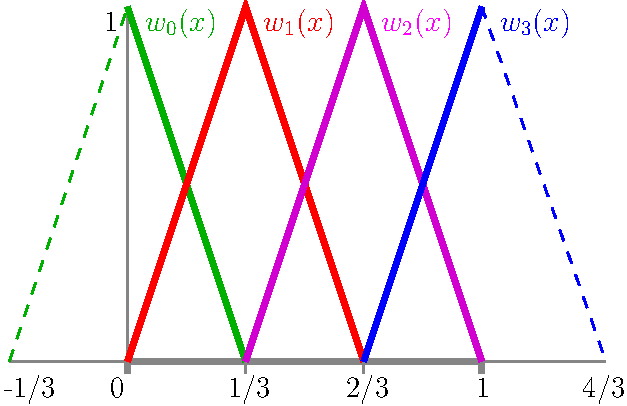
\includegraphics[width=.3\linewidth]{blending_functions.pdf}
	\caption{Hat function basis for FEM approximation.}
	\label{fig:fem:blending}
\end{figure}

This choice is somewhat arbitrary, there are numerous possible bases.
Then the approximate solution is a linear combination of the weighting functions:
$$
\tilde{\varphi}(x) := 0\cdot w_0(x) + b\cdot w_1(x) + c\cdot w_2(x) + 1\cdot w_3(x),
$$
where the coefficients of $w_0(x)$ and $w_3(x)$ are the direct consequence of the boundary condition $\varphi(0)=0$, $\varphi(1)=1$;
note that $b$ and $c$ give the values of the approximation for the points $x=\frac{1}{3}$ and $x=\frac{2}{3}$, respectively.

With a differential equation we do not know how to measure the true error, 
so we must instead require the residual $\frac{d^2\tilde{\varphi}}{dx^2} - f$ to be orthogonal to $\Span\{w_1,\dots w_{n-1}\}$.

\TODO{explanation, figure, residual orthogonal to the solution space}


The residual being orthogonal to the solution space can be written as follows:
$$
\int\limits_0^1 w_i \cdot \left(\frac{d^2\tilde{\varphi}}{dx^2} - f\right) dx = 0, \quad i = 1\dots n-1 
$$

Note that $w_i(x)$ is equal to zero outside the interval $[x_{i-1}, x_{i+1}]$, this allows us to rewrite the system:
$$
\int\limits_{x_{i-1}}^{x_{i+1}} w_i \cdot \frac{d^2\tilde{\varphi}}{dx^2}\,dx - \int\limits_{x_{i-1}}^{x_{i+1}} w_i\cdot f\,dx = 0, \quad i = 1\dots n-1
$$

Most often both integrals are evaluated numerically, or symbolic calculations are peformed over the left integral only.
The left integral is a dot product between the basis functions and the differential operator defined on a combination of basis functions;
it depends on the choice of the basis and can be precomputed.
As our problem is very simple, we will find the solution symbolically.

Attention! The next step will be done on a slippery ground.
Our weighting functions are not differentiable everywhere, and caution must be taken.
Anyhow, let us integrate by parts the first integral:
\begin{align*}
\int\limits_{x_{i-1}}^{x_{i+1}} w_i \cdot \frac{d^2\tilde{\varphi}}{dx^2}\,dx &= 
\int\limits_{x_{i-1}}^{x_{i}} w_i \cdot \frac{d^2\tilde{\varphi}}{dx^2}\,dx + 
\int\limits_{x_{i}}^{x_{i+1}} w_i \cdot \frac{d^2\tilde{\varphi}}{dx^2}\,dx = \\
& =\underbrace{\lim\limits_{\varepsilon\rightarrow 0}w_i\cdot \frac{d\tilde{\varphi}}{dx}\Big|_{x_{i-1}+\varepsilon}^{x_{i}-\varepsilon} +
\lim\limits_{\varepsilon\rightarrow 0}w_i\cdot \frac{d\tilde{\varphi}}{dx}\Big|_{x_{i}+\varepsilon}^{x_{i+1}-\varepsilon}}_{= 0} - \int\limits_{x_{i-1}}^{x_{i+1}} \frac{dw_i}{dx}\cdot \frac{d\tilde{\varphi}}{dx}\,dx  = \\
& = - \int\limits_{x_{i-1}}^{x_{i+1}} \frac{dw_i}{dx}\cdot \frac{d\tilde{\varphi}}{dx}\,dx \\
\end{align*}

It allows us to rewrite the system of equations:
\begin{equation}
\label{eq:galerkin:system}
\int\limits_{x_{i-1}}^{x_{i+1}} \frac{dw_i}{dx} \cdot \frac{d\tilde{\varphi}}{dx}\,dx + \int\limits_{x_{i-1}}^{x_{i+1}} w_i\cdot f\,dx = 0, \quad i = 1\dots n-1
\end{equation}

$$
\frac{d\tilde{\varphi}}{dx} (x) := \left\{
\begin{split}
3b, & \quad 0 < x < \frac{1}{3}\\
-3b+3c, & \quad \frac{1}{3} < x < \frac{2}{3}\\
-3c+3, & \quad \frac{2}{3} < x < 1\\
0 & \quad \text{otherwise}
\end{split}
\right.
$$

$$
\frac{dw_1}{dx} (x) := \left\{
\begin{split}
3, & \quad 0 < x < \frac{1}{3}\\
-3, & \quad \frac{1}{3} < x < \frac{2}{3}\\
0 & \quad \text{otherwise}
\end{split}
\right.
$$

$$
\frac{dw_2}{dx} (x) := \left\{
\begin{split}
3, & \quad \frac{1}{3} < x < \frac{2}{3}\\
-3, & \quad \frac{2}{3} < x < 1\\
0 & \quad \text{otherwise}
\end{split}
\right.
$$

Then the system~\eqref{eq:galerkin:system} can be rewritten as follows:

$$
\left\{
\begin{split}
\int\limits_{0}^{1/3} 3\cdot 3b\,dx + \int\limits_{1/3}^{2/3} -3\cdot (-3b+3c)\, dx + \int\limits_{0}^{1/3} 3x(x+1)\,dx + \int\limits_{1/3}^{2/3}(2-3x)(x+1)\,dx &= 0\\
\int\limits_{1/3}^{2/3} 3\cdot (-3b+3c)\,dx + \int\limits_{2/3}^{1} -3\cdot (-3c+3)\, dx + \int\limits_{1/3}^{2/3} (3x-1)(x+1)\,dx + \int\limits_{2/3}^{1}(3-3x)(x+1)\,dx &= 0\\
\end{split}
\right.
$$

$$
\left\{
\begin{split}
2b - c &= -\frac{4}{27}\\
-b + 2c &= \frac{22}{27}
\end{split}
\right.
$$

$b=\frac{14}{81}$, $c=\frac{40}{81}$
\begin{figure}[ht]
	\centering
	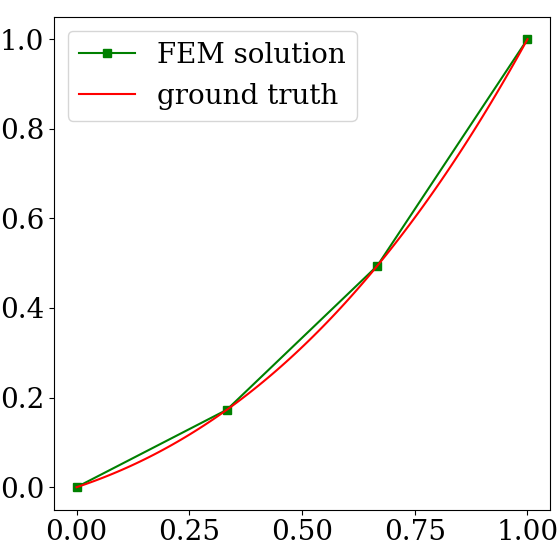
\includegraphics[width=.3\linewidth]{fem}
	\caption{The ground truth $\varphi(x) = \frac{1}{6} x^3 + \frac{1}{2} x^2 + \frac{1}{3} x$ and its approximation found by the FEM.}
	\label{fig:fem}
\end{figure}

\TODO{Mention Ritz and guide towards least squares}





\chapter{Minimization of quadratic functions and linear systems}

Recall that the main goal is to study least squares, therefore our main tool will be the minimization of quadratic functions;
however, before we start using this power tool, we need to find where its on/off button is located.
First of all, we need to recall what a matrix is; then we will revisit the definition of a positive numbers, and only then we will attack minimization of quadratic functions.

\section{Matrices and numbers}
In this sections, matrices will be omnipresent, so let's remember what it is.
Do not peek further down the text, pause for a few seconds, and try to formulate what the matrix is.

\subsection{Different interpretations of matrices}

The answer is very simple. A matrix is just a locker that stores stuff.
Each piece of stuff lies in its own cell, cells are grouped in rows and columns.
In our particular case, we store real numbers; for a programmer the easiest way to imagine a matrix $A$ is something like:
\begin{minted}{cpp}
float A[m][n];
\end{minted}

Why would we need a storage like this? What does it describe?
Maybe I will upset you, but the matrix by itself does not describe anything, it stores stuff.
For example, you can store coefficients of a function in it.
Let us put aside matrices for a second imagine that we have a number $a$. What does it mean?
Who knows what it means\dots For example, it can be a coefficient inside a function that takes one number as an input and gives another number as an output:
$$
f(x) : \mathbb R \rightarrow \mathbb R
$$

One possible instance of such a function a mathematicion could write down as:
$$
f(x) = ax
$$

In the programmers' world it would look something like this:
\begin{minted}[linenos=true]{cpp}
float f(float x) {
    return a*x;
}
\end{minted}

On the other hand, why this function and not another one? Let's take another one!
$$
f(x) = ax^2
$$
A programmer would write it like this:
\begin{minted}[linenos=true]{cpp}
float f(float x) {
    return x*a*x;
}
\end{minted}

One of these functions is linear and the other is quadratic. Which one is correct? 
Neither one. The number $a$ does not define it, it just stores a value! 
Build the function you need.

The same thing happens to matrices, they give storage space when simple numbers (scalars) do not suffice, a matrix is a sort of an hyper-number.
The addition and multiplication operations are defined over matrices just as over numbers.
%. The division is a bit more complicated, but in certain cases it can be defined too.

Let us suppose that we have a $2\times 2$ matrix $A$:
$$
A=\begin{bmatrix} a_{11} & a_{12} \\ a_{21} & a_{22}\end{bmatrix}
$$

The matrix does not mean anything by itself, for example, it can be interpreted as a linear function:
$$
f(x) : \mathbb R^2 \rightarrow \mathbb R^2, \quad f(x) = Ax
$$

Here goes the programmer's view on the function:
\begin{minted}[linenos=true]{cpp}
vector<float> f(vector<float> x) {
    return vector<float>{a11*x[0] + a12*x[1],  a21*x[0] + a22*x[1]};
}
\end{minted}

This function maps a two-dimensional vector to a two-dimensional vector.
Graphically, it is convenient to imagine it as an image transformation: we give an input image, and the output is the stretched and/or rotated (maybe even mirrored!) version.
The top row of Figure~\ref{fig:matrices} provides few different examples of this interpretation of matrices.

On the other hand, nothing prevents to interpret the matrix $A$ as a function that maps a vector to a scalar:
$$
f(x) : \mathbb R^2 \rightarrow \mathbb R, \quad f(x) = x^\top A x = \sum\limits_i\sum\limits_j a_{ij}x_i x_j
$$

Note that the square is not very well defined for the vectors, so I cannot write $x^2$ as I wrote in the case of ordinary numbers. 
For those who are not at ease with matrix multiplications, I highly recommend to revisit it right now and check that the expression $x^\top A x$ indeed produces a scalar value.
To this end, we can explicitly put brackets $x^\top A x = (x^\top A) x$.
Recall that in this particular example $x$ is a two-dimensional vector (stored in a $2\times 1$ matrix).
Let us write all the matrix dimensions explicitly:
$$
\underbrace{\underbrace{\left(\underbrace{x^\top}_{1\times 2} \times \underbrace{A}_{2\times 2}\right)}_{1\times 2} \times \underbrace{x}_{2\times 1}}_{1 \times 1}
$$

Returning to the cozy world of programmers, we can write the same quadratic function as follows:
\begin{minted}[linenos=true]{cpp}
float f(vector<float> x) {
    return x[0]*a11*x[0] + x[0]*a12*x[1] + x[1]*a21*x[0] + x[1]*a22*x[1];
}
\end{minted}

\begin{figure}[ht]
	\centering
	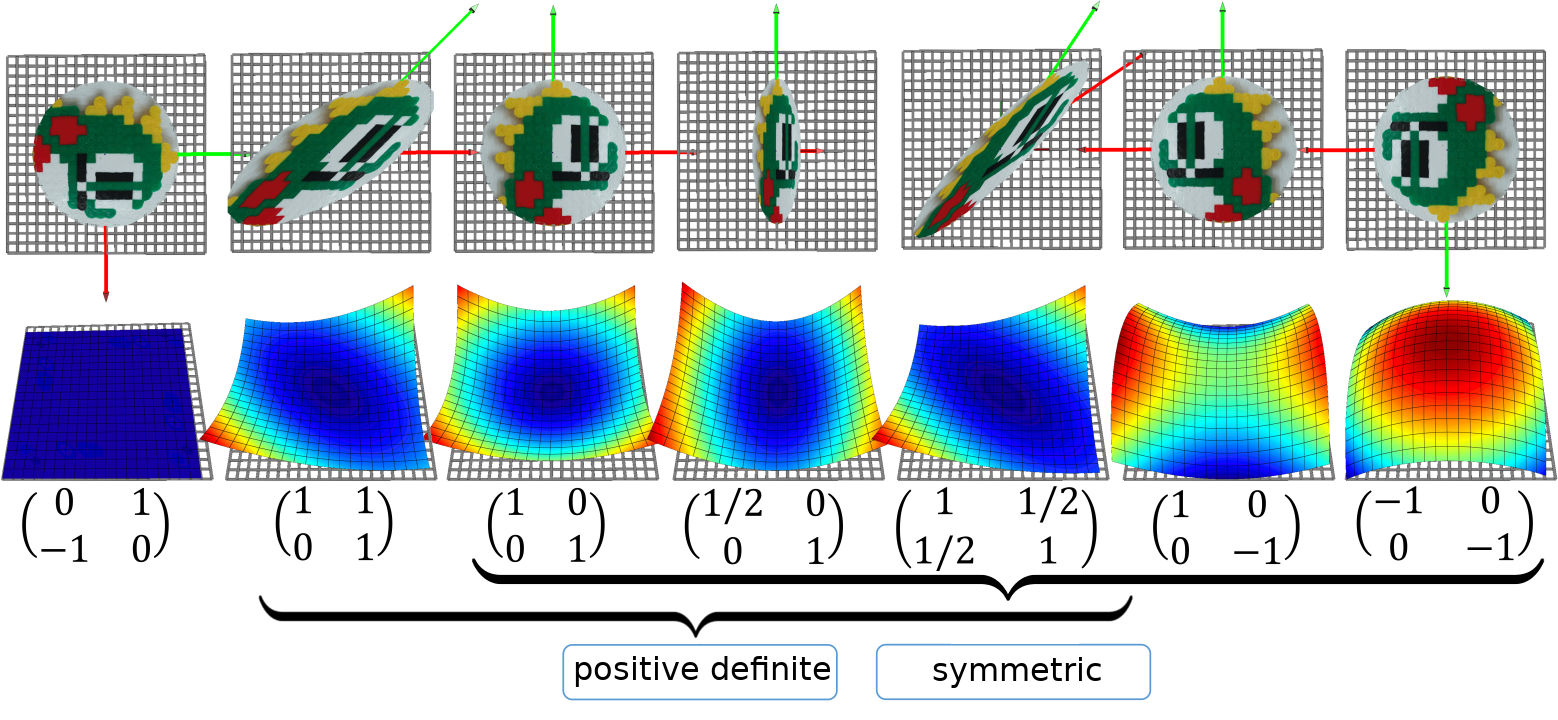
\includegraphics[width=\linewidth]{matrices}
	\caption{Seven examples of $2\times 2$ matrices, some of them are positive definite and/or symmetric. 
    \textbf{Top row:} the matrices are interpreted as linear functions $f(x):\mathbb R^2 \rightarrow \mathbb R^2$. \textbf{Middle row:} the matrices are interpreted as quadratic functions
 $f(x):\mathbb R^2 \rightarrow \mathbb R$.}
	\label{fig:matrices}
\end{figure}


\subsection{What is a positive number?}
Allow me to ask a very stupid question: what is a positive number?
We have a great tool called the predicate ``greater than'' $>$.
Do not be in a hurry to answer that the number $a$ is positive if and only if $a>0$, it would be too easy. Let us define the positivity as follows:

\begin{definition}
The real number $a$ is positive if and only if for all non-zero real $x\in\mathbb R,\ x\neq 0$ the condition $ax^2>0$ is satisfied.
\end{definition}

Looks pretty awkward, but it applies perfectly to the matrices:

\begin{definition}
The square matrix $A$ is called positive definite if for any non-zero $x$
the condition $x^\top A x > 0$ is met, i.e. the corresponding quadratic form is strictly positive everywhere except at the origin.
\end{definition}

What do we need the positivity for?
As we have already mentioned, our main tool will be the minimization of quadratic functions. 
It would be nice to be sure that the minimum exists!
For example, the function $f(x) = - x^2$ clearly has no minimum, because the number -1 is not positive, 
both branches of the parabola $f(x)$ look down.
Positive definite matrices guarantee that the corresponding quadratic forms form a paraboloid with a (unique) minimum.
Refer to the Figure~\ref{fig:matrices} for an illustration.

Thus, we will work with a generalization of positive numbers, namely, positive definite matrices. 
Moreover, in our particular case, the matrices will be symmetric!
Note that quite often, when people talk about positive definiteness, they also imply symmetry.
This can be partly explained by the following observation (optional for the understanding of the rest of the text):

\subsubsection{A digression on quadratic forms and matrix symmetry}

Let us consider a quadratic form $x^\top M x$ for an arbitrary matrix $M$. 
Next we add and subtract a half ot its transpose:
$$
M = \underbrace{\frac{1}{2} (M+M^\top)}_{:=M_s} + \underbrace{\frac{1}{2} (M-M^\top)}_{:=M_a} = M_s + M_a
$$

The matrix $M_s$ is symmetric: $M_s^\top = M_s$; the matrix $M_a$ is antisymmetric: $M_a^\top=-M_a$.
A remarkable fact is that for any antisymmetric matrix the corresponding quadratic form is equal to zero everywhere. This follows from the following observation:
$$
q = x^\top M_a x  = (x^\top M_a^\top x)^\top = - (x^\top M_a x)^\top = -q
$$
It means that the quadratic form $x^\top M_a x$ equals $q$ and $-q$ at the same time, and the only way to have this condition is to have $q\equiv 0$.
From this fact it follows that for an arbitrary matrix $M$ the corresponding quadratic form $x^\top M x$ can be expressed through the symmetric matrix $M_s$ as well:
$$
x^\top M x = x^\top (M_s + M_a) x = x^\top M_s x  + x^\top M_a x = x^\top M_s x.
$$


\section{Minimizing a quadratic function}

\begin{figure}[ht]
	\centering
	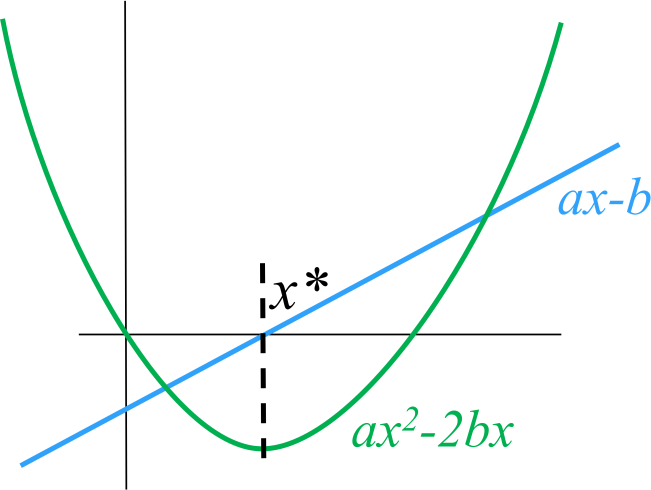
\includegraphics[width=.3\linewidth]{minpb1d}
	\caption{In 1d, the solution $x^*$ of the equation $ax - b = 0$ solves the minimization problem $\argmin\limits_x(ax^2-2bx)$ as well. }
	\label{fig:min1d}
\end{figure}

Let us return to the one-dimensional world for a while; I want to find the minimum of the function $f(x) = ax^2 - 2bx$. 
The number $a$ is positive, therefore the minimum exists; to find it, we equate with the corresponding derivative with zero: $\frac{d}{dx}f(x) = 0$. 
It is easy to differentiate a one-dimensional quadratic function: $\frac{d}{dx}f(x) = 2ax - 2b = 0$; so our problem boils down to the equation $ax-b=0$.
With some effort we can find the solution $x^* = b/a$. Figure~\ref{fig:min1d} illustrates the equivalence of two problems:
the solution $x^*$ of the equation $ax-b=0$ coincides with the minimizer $\argmin\limits_x(ax^2 - 2bx)$.

My point is that our main goal is to minimize quadratic functions (we are talking about least squares here!).
The only thing that the humanity knows to do well is to solve linear equations, and it is great that one is equivalent to the other!
The last thing is to check whether this equivalence holds for the case of $n>1$ variables.
To do so, we will first prove three theorems.

\subsection{Three theorems, or how to differentiate matrix expressions}
The first theorem states that $1\times 1$ matrices are invariant w.r.t the transposition:
\begin{theorem}
$x\in \mathbb R \Rightarrow x^\top = x$
\end{theorem}
The proof is left as an exercise.

The second theorem allows us to differentiate linear functions. In the case of a real function of one variable we know that
$\frac{d}{dx}(bx) = b$, but what happens in the case of a real function of $n$ variables?
\begin{theorem}
$\nabla b^\top x = \nabla x^\top b = b$
\end{theorem}
No surprises here, the same result in a matrix notation. The proof is straightforward, it suffices to write down the definition of the gradient:
$$\nabla(b^\top x) = \begin{bmatrix}\frac{\partial (b^\top x)}{\partial x_1} \\ \vdots \\ \frac{\partial (b^\top x)}{\partial x_n} \end{bmatrix} = \begin{bmatrix}\frac{\partial (b_1 x_1 + \dots + b_n x_n)}{\partial x_1} \\ \vdots \\ \frac{\partial (b_1 x_1 + \dots + b_n x_n)}{\partial x_n} \end{bmatrix}
= \begin{bmatrix}b_1 \\ \vdots \\ b_n \end{bmatrix} = b$$
Now applying the first theorem: $b^\top x = x^\top b$, and this concludes the proof.

Now let us switch to quadratic forms.
We know that in the case of a real function of one variable we have $\frac{d}{dx}(ax^2) = 2ax$, but what happens with the quadratic forms?
\begin{theorem}
$\nabla (x^\top A x) = (A+A^\top)x$
\end{theorem}
Note that if $A$ is symmetric, then $\nabla (x^\top A x) = 2Ax$.
The proof is straightforward, let us express the quadratic form as a double sum:
$$x^\top A x = \sum\limits_i\sum\limits_j a_{ij} x_i x_j$$
Now let us differentiate this double sum w.r.t the variable $x_i$:
\begin{align*}
\frac{\partial (x^\top A x)}{\partial x_i} 
&= \frac{\partial}{\partial x_i}  \left(\sum\limits_{k_1}\sum\limits_{k_2} a_{k_1 k_2} x_{k_1} x_{k_2}\right) = \\
&= \frac{\partial}{\partial x_i}  \left(
\underbrace{\sum\limits_{k_1\neq i}\sum\limits_{k_2\neq i} a_{ik_2}x_{k_1} x_{k_2}}_{k_1 \neq i, k_2 \neq i}+\underbrace{\sum\limits_{k_2\neq i} a_{ik_2}x_i x_{k_2}}_{k_1 = i, k_2\neq i}+
\underbrace{\sum\limits_{k_1\neq i} a_{k_1 i} x_{k_1} x_i}_{k_1 \neq i, k_2 = i}+
\underbrace{a_{ii}x_i^2}_{k_1 = i, k_2 = i}\right) = \\
& = \sum\limits_{k_2\neq i} a_{ik_2}x_{k_2} + \sum\limits_{k_1\neq i} a_{k_1 i} x_{k_1} + 2 a_{ii} x_i = \\
& = \sum\limits_{k_2} a_{ik_2}x_{k_2} + \sum\limits_{k_1} a_{k_1 i} x_{k_1} = \\
& = \sum\limits_{j} (a_{ij} + a_{ji}) x_j \\
\end{align*}
I split the double sum into four cases, shown by the curly brackets.
Each of these four cases is trivial to differentiate. 
Now let us collect the partial derivatives  into a gradient vector:
$$\nabla(x^\top A x) = \begin{bmatrix}\frac{\partial (x^\top Ax)}{\partial x_1} \\ \vdots \\ \frac{\partial (x^\top A x)}{\partial x_n} \end{bmatrix}  = \begin{bmatrix}\sum\limits_{j} (a_{1j} + a_{j1}) x_j \\ \vdots \\ \sum\limits_{j} (a_{nj} + a_{jn}) x_j \end{bmatrix}  = (A+A^\top)x
$$

\subsection{Minimum of a quadratic function and the linear system}
Recall that for a positive real number $a$ solving the equation
$ax=b$ is equivalent to the quadratic function $\argmin\limits_x(ax^2 - 2bx)$ minimization.

We want to show the corresponding connection in the case of a symmetric positive definite matrix $A$.
So, we want to find the minimum quadratic function
$$\argmin\limits_{x\in\mathbb R^n} (x^\top A x - 2b^\top x).$$
As before, let us equate the derivative to zero:
$$\nabla (x^\top A x - 2b^\top x) = \begin{bmatrix}0 \\ \vdots \\ 0 \end{bmatrix}.$$
The Hamilton operator is linear, so we can rewrite our equation as follows:
$$\nabla (x^\top A x) - 2\nabla(b^\top x) = \begin{bmatrix}0 \\ \vdots \\ 0 \end{bmatrix}.$$
Now let us apply the second and third differentiation theorems:
$$(A+A^\top)x - 2b = \begin{bmatrix}0 \\ \vdots \\ 0 \end{bmatrix}.$$
Recall that $A$ is symmetric, let us divide the equation by 2, and we obtain the final linear system:
$$Ax = b.$$
Hurray, passing from one variable to many, we have not lost a thing, and can effectively minimize quadratic functions!

%$$\argmin (x^\top A x - 2b^\top x) = A^{-1}b$$

\section{Переходим к наименьшим квадратам}
Наконец мы можем перейти к основному содержанию этой лекции. Представьте, что у нас есть две точки на плоскости $(x_1, y_1)$ и $(x_2, y_2)$, и мы хотим найти уравнение прямой, проходящей через эти две точки.
Уравнение прямой можно записать в виде $y = \alpha x + \beta$, то есть, наша задача это найти коэффициенты $\alpha$ и $\beta$. Это упражнение для седьмого-восьмого класса школы, запишем систему уравнений:
$$
\left\{
\begin{split}
\alpha x_1 + \beta &= y_1\\
\alpha x_2 + \beta &= y_2\\
\end{split}
\right.
$$

У нас два уравнения с двумя неизвестными ($\alpha$ и $\beta$), остальное известно.
В общем случае решение существует и единственно. Для удобства перепишем ту же самую систему в матричном виде:
$$
\underbrace{\begin{bmatrix}x_1  & 1 \\ x_2 & 1 \end{bmatrix}}_{:=A} 
\underbrace{\begin{bmatrix} \alpha \\ \beta \end{bmatrix}}_{:=x} = \underbrace{\begin{bmatrix} y_1 \\ y_2 \end{bmatrix}}_{:=b}
$$

Получим уравнение типа $Ax = b$, которое тривиально решается $x^* = A^{-1}b$.

А теперь представим, что у нас есть \textbf{три} точки, через которые нужно провести прямую:
$$
\left\{
\begin{split}
\alpha x_1 + \beta &= y_1\\
\alpha x_2 + \beta &= y_2\\
\alpha x_3 + \beta &= y_3\\
\end{split}
\right.
$$

В матричном виде эта система запишется следующим образом:
$$
\underbrace{\begin{bmatrix}x_1  & 1 \\ x_2 & 1 \\x_3 & 1 \end{bmatrix} }_{:= A\,(3\times 2)}
\underbrace{\begin{bmatrix} \alpha \\ \beta \end{bmatrix}}_{:=x\,(2\times 1)} = \underbrace{\begin{bmatrix} y_1 \\ y_2 \\ y_3 \end{bmatrix}}_{:=b\, (3\times 1)}
$$
Теперь у нас матрица $A$ прямоугольная, и у неё просто не существует обратной! Это совершенно нормально, так как у нас всего две переменных и три уравнения, и в общем случае эта система не имеет решения.
Это соверешенно нормальная ситуация в реальном мире, когда точки - это данные зашумлённых измерений, и нам нужно найти параметры $\alpha$ и $\beta$, которые наилучшим образом \textit{приближают} данные измерений.
Мы этот пример уже рассматривали в первой лекции, когда калибровали безмен. Но тогда у нас решение было чисто алгебраическим и очень громоздким. Давайте попробуем более интуитивный способ.

Нашу систему можно записать в следующем виде:
$$
\alpha \underbrace{\begin{bmatrix}x_1  \\ x_2 \\x_3  \end{bmatrix} }_{:=\vec{i}}
+\beta \underbrace{\begin{bmatrix}1 \\ 1 \\1 \end{bmatrix} }_{:=\vec{j}} = 
\begin{bmatrix}y_1\\y_2\\y_3\end{bmatrix}
$$
Или, более кратко, 
$$
\alpha \vec{i} + \beta\vec{j} = \vec{b}.
$$
Векторы $\vec i$, $\vec j$ и $\vec b$ известны, нужно найти скаляры $\alpha$ и $\beta$.
Очевидно, что линейная комбинация $\alpha \vec{i} + \beta\vec{j}$ порождает плоскость, и если вектор $\vec b$ в этой плоскости не лежит, то точного решения не существует; однако же мы ищем приближённое решение.

Давайте определим ошибку решения как $\vec{e}(\alpha, \beta) :=  \alpha \vec{i} + \beta\vec{j} - \vec b$.
Нашей зачей является найти такие значения параметров $\alpha$ и $\beta$, которые минимизируют длину вектора $\vec{e}(\alpha, \beta)$. Иначе говоря, проблема записывается как $\argmin\limits_{\alpha, \beta} \|\vec{e}(\alpha, \beta)\|$.
Иллюстрация дана на рисунке~\ref{fig:error}.

\begin{figure}[ht]
	\centering
	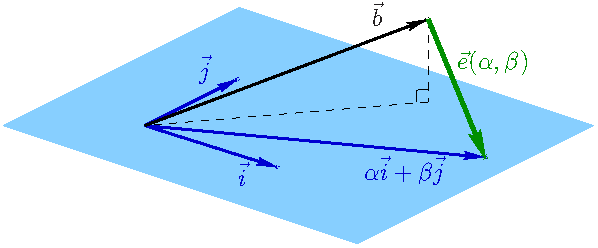
\includegraphics[width=.7\linewidth]{error.pdf}
	\caption{Имея заданные векторы $\vec i$, $\vec j$ и $\vec b$, мы стараемся минимизировать длину вектора ошибки $\vec e$. Очевидно, что его длина минимизируется, если он перпендикулярен плоскости, натянутой на векторы $\vec i$ и $\vec j$.}
	\label{fig:error}
\end{figure}

Но постойте, где же наименьшие квадраты? Сейчас будут. Функция извлечения корня $\sqrt{\cdot}$ монотонна, поэтому $\argmin\limits_{\alpha, \beta} \|\vec{e}(\alpha, \beta)\|$ = $\argmin\limits_{\alpha, \beta} \|\vec{e}(\alpha, \beta)\|^2$!

Вполне очевидно, что длина вектора ошибки минимизируется, если он перпендикулярен плоскости, натянутой на векторы $\vec i$ и $\vec j$, что можно записать, приравняв нулю соответствующие скалярные произведения:

$$
\left\{
\begin{split}\vec{i}^\top \vec{e}(\alpha, \beta) &= 0\\
\vec{j}^\top \vec{e}(\alpha, \beta) &= 0
\end{split}
\right.
$$

В матричном виде эту же самую систему можно записать как
$$
\begin{bmatrix}x_1 & x_2 & x_3 \\ 1 & 1 & 1 \end{bmatrix}
\left(\alpha \begin{bmatrix}x_1  \\ x_2 \\x_3  \end{bmatrix}
+\beta \begin{bmatrix}1 \\ 1 \\1 \end{bmatrix} - 
\begin{bmatrix}y_1\\y_2\\y_3\end{bmatrix}\right) = \begin{bmatrix}0\\0\end{bmatrix}
$$
или же
$$
\begin{bmatrix}x_1 & x_2 & x_3 \\ 1 & 1 & 1 \end{bmatrix}
\left(
\begin{bmatrix}x_1  & 1 \\ x_2 & 1 \\x_3 & 1 \end{bmatrix}
\begin{bmatrix} \alpha \\ \beta \end{bmatrix}-
\begin{bmatrix} y_1 \\ y_2 \\ y_3 \end{bmatrix}
\right) = \begin{bmatrix}0\\0\end{bmatrix}
$$
Но мы на этом не остановимся, так как запись можно ещё больше сократить:
$$
A^\top (Ax - b)= \begin{bmatrix}0\\0\end{bmatrix}
$$
И самая последняя трансформация:
$$
A^\top Ax = A^\top b.
$$
Давайте посчитаем размерности. Матрица $A$ имеет размер $3\times 2$, поэтому $A^\top A$ имеет размер $2\times 2$. Матрица $b$ имеет размер $3\times 1$, но вектор $A^\top b$ имеет размер $2\times 1$.
То есть, в общем случае матрица $A^\top A$ обратима! Более того, $A^\top A$ имеет ещё пару приятных свойств.

\begin{theorem}
$A^\top A$ симметрична.
\end{theorem}
Это совсем нетрудно показать:
$$
(A^\top A)^\top = A^\top (A^\top)^\top = A^\top A.
$$

\begin{theorem}
	$A^\top A$ положительно полуопределена: $\forall x\in \mathbb R^n\quad x^\top A^\top A x \geq 0.$
\end{theorem}
Это следует из того факта, что $x^\top A^\top A x = (A x)^\top A x > 0$.

Кроме того, $A^\top A$ положительно определена в том случае, если $A$ имеет линейно независимые столбцы (ранг $A$ равен количеству переменных в системе).

\vspace{5mm}

Итого, для системы с двумя неизвестными мы доказали, что минимизация 
квадратичной функции $\argmin\limits_{\alpha, \beta} \|\vec{e}(\alpha, \beta)\|^2$ эквивалентна решению системы линейных уравнений $A^\top A x = A^\top b$. Разумеется, всё это рассуждение применимо и к любому другому количеству переменных, но давайте ещё раз компактно запишем всё вместе простым алгебраическим подсчётом.
Мы начнём с проблемы наименьших квадратов, придём к минимизации квадратичной функции знакомого нам вида,
и из этого сделаем вывод об эквивалентности решению системы линейных уравнений. Итак, поехали:
\begin{align*}
\argmin \| Ax - b \|^2 &= \argmin (Ax-b)^\top (Ax-b) =\\
& = \argmin(x^\top A^\top - b^\top)(Ax-b) = \\
& = \argmin(x^\top A^\top A x - b^\top Ax - x^\top A^\top b + \underbrace{b^\top b}_{\rm const})=\\
& = \argmin(x^\top A^\top A x - 2b^\top Ax) = \\
& = \argmin(x^\top \underbrace{(A^\top A)}_{:=A'} x - 2\underbrace{(A^\top b)}_{:=b'}\phantom{}^\top x)
\end{align*}
Таким образом, проблема наименьших квадратов $\argmin \| Ax - b \|^2$  эквивалентна минимизации квадратичной функции $\argmin (x^\top A' x - 2b'^\top x)$ с (в общем случае) симметричной положительно определённой матрицей $A'$, что, в свою очередь, эквивалентно решению системы линейных уравнений $A'x = b'$. Уфф. Теория закончилась.


%\chapter{Finite elements example: the Ritz method}


\chapter{Conjugate gradient for geometry processing}

\begin{equation}
\nonumber
\resizebox{\hsize}{!}{
$\left\{
\begin{array}{cccccccccccccccccl}
2x_1  & -x_2  &       &         &        &          &           &          &                   &            &          &         &        &          &          &          &                   &= x_0 \\
-x_1  & +2x_2 & -x_3  &         &        &          &           &          &                   &            &          &         &        &          &          &          &                   &= 0 \\
      & -x_2  & +2x_3 & -x_4    &        &          &           &          &                   &            &          &         &        &          &          &          &                   &= 0 \\
      &       &       &         & \ddots &          &           &          &                   &            &          &         &        &          &          &          &                   &  \vdots \\
      &       &       &         &        &  -x_{15} &  +2x_{16} & -x_{17}  &                   &            &          &         &        &          &          &          &                   &= 0      \\
      &       &       &         &        &          &  -x_{16}  & +2x_{17} &                   &            &          &         &        &          &          &          &                   &= x_{18} \\
      &       &       &         &        &          &           &          &          +2x_{19} & -x_{20}    &          &         &        &          &          &          &                   &= x_{18} \\
      &       &       &         &        &          &           &          &           -x_{19} & +2x_{20}   & -x_{21}  &         &        &          &          &          &                   &= 0 \\
      &       &       &         &        &          &           &          &                   &            &          &  \ddots &        &          &          &          &                   &  \vdots \\
      &       &       &         &        &          &           &          &                   &            &          &         &        & -x_{27}  & +2x_{28} & -x_{29}  &                   &= 0 \\
      &       &       &         &        &          &           &          &                   &            &          &         &        &          & -x_{28}  & +2x_{29} & -x_{30}           &= 0 \\
      &       &       &         &        &          &           &          &                   &            &          &         &        &          &          & -x_{29}  & +2x_{30}          &= x_{31} \\
\end{array}
\right.$
}
\end{equation}



\begin{equation}
\nonumber
\resizebox{\hsize}{!}{
$\left\{
\begin{array}{|c|ccccccc|c|ccccccc|c|c}
-x_0 & +x_1  &      &      &         &        &            &         &         &         &            &        &            &         &         &         &         &= 0 \\
     &  -x_1 & +x_2 &      &         &        &            &         &         &         &            &        &            &         &         &         &         &= 0 \\
     &       & -x_2 & +x_3 &         &        &            &         &         &         &            &        &            &         &         &         &         &= 0 \\
     &       &      & -x_3 & +x_4    &        &            &         &         &         &            &        &            &         &         &         &         &= 0 \\
     &       &      &      &         & \ddots &            &         &         &         &            &        &            &         &         &         &         &  \vdots  \\
     &       &      &      &         &        &    -x_{16} & +x_{17} &         &         &            &        &            &         &         &         &         &= 0 \\
     &       &      &      &         &        &            & -x_{17} & +x_{18} &         &            &        &            &         &         &         &         &= 0 \\
     &       &      &      &         &        &            &         & -x_{18} & +x_{19} &            &        &            &         &         &         &         &= 0 \\
     &       &      &      &         &        &            &         &         & -x_{19} & +x_{20}    &        &            &         &         &         &         &= 0 \\
     &       &      &      &         &        &            &         &         &         &            & \ddots &            &         &         &         &         &  \vdots  \\
     &       &      &      &         &        &            &         &         &         &            &        &    -x_{27} & +x_{28} &         &         &         &= 0 \\
     &       &      &      &         &        &            &         &         &         &            &        &            & -x_{28} & +x_{29} &         &         &= 0 \\
     &       &      &      &         &        &            &         &         &         &            &        &            &         & -x_{29} & +x_{30} &         &= 0 \\
     &       &      &      &         &        &            &         &         &         &            &        &            &         &         & -x_{30} & +x_{31} &= 0 \\
\end{array}
\right.$
}
\end{equation}

\begin{equation}
\nonumber
\resizebox{\hsize}{!}{
$\left\{
\begin{array}{ccccccccccccccl}
       +x_1  &      &      &         &        &            &         &                   &            &        &            &         &         &                   &= +x_0 \\
        -x_1 & +x_2 &      &         &        &            &         &                   &            &        &            &         &         &                   &= 0 \\
             & -x_2 & +x_3 &         &        &            &         &                   &            &        &            &         &         &                   &= 0 \\
             &      & -x_3 & +x_4    &        &            &         &                   &            &        &            &         &         &                   &= 0 \\
             &      &      &         & \ddots &            &         &                   &            &        &            &         &         &                   &  \vdots  \\
             &      &      &         &        &    -x_{16} & +x_{17} &                   &            &        &            &         &         &                   &= 0 \\
             &      &      &         &        &            & -x_{17} &                   &            &        &            &         &         &                   &= -x_{18} \\
             &      &      &         &        &            &         &           +x_{19} &            &        &            &         &         &                   &= +x_{18} \\
             &      &      &         &        &            &         &           -x_{19} & +x_{20}    &        &            &         &         &                   &= 0 \\
             &      &      &         &        &            &         &                   &            & \ddots &            &         &         &                   &  \vdots  \\
             &      &      &         &        &            &         &                   &            &        &    -x_{27} & +x_{28} &         &                   &= 0 \\
             &      &      &         &        &            &         &                   &            &        &            & -x_{28} & +x_{29} &                   &= 0 \\
             &      &      &         &        &            &         &                   &            &        &            &         & -x_{29} & +x_{30}           &= 0 \\
             &      &      &         &        &            &         &                   &            &        &            &         &         & -x_{30}           &= -x_{31} \\
\end{array}
\right.$
}
\end{equation}

\begin{equation}
\nonumber
\resizebox{\hsize}{!}{
$\left\{
\begin{array}{cccccccccccccccccl}
-x_0 & +x_1  &      &      &         &        &            &         &         &         &            &        &            &         &         &         &         &= 0 \\
     &  -x_1 & +x_2 &      &         &        &            &         &         &         &            &        &            &         &         &         &         &= 0 \\
     &       &      &      &         & \ddots &            &         &         &         &            &        &            &         &         &         &         &  \vdots   \\
     &       &      &      &         &        &    -x_{16} & +x_{17} &         &         &            &        &            &         &         &         &         &= 0 \\
     &       &      &      &         &        &            & -x_{17} & +x_{18} &         &            &        &            &         &         &         &         &= 0 \\
     &       &      &      &         &        &            &         & -x_{18} & +x_{19} &            &        &            &         &         &         &         &= 0 \\
     &       &      &      &         &        &            &         &         & -x_{19} & +x_{20}    &        &            &         &         &         &         &= 0 \\
     &       &      &      &         &        &            &         &         &         &            & \ddots &            &         &         &         &         &  \vdots  \\
     &       &      &      &         &        &            &         &         &         &            &        &            &         & -x_{29} & +x_{30} &         &= 0 \\
     &       &      &      &         &        &            &         &         &         &            &        &            &         &         & -x_{30} & +x_{31} &= 0 \\
100\cdot x_{0}     &       &      &      &         &        &            &         &         &         &            &        &            &         &         &         &  &= 100\cdot 1 \\
     &       &      &      &         &        &            &         & 100\cdot x_{18} &         &            &        &            &         &         &         &         &= 100\cdot 2 \\
     &       &      &      &         &        &            &         &         &         &            &        &            &         &         &         & 100\cdot x_{31} &= 100\cdot 1 \\
\end{array}
\right.$
}
\end{equation}



\begin{figure}[ht]
	\centering
    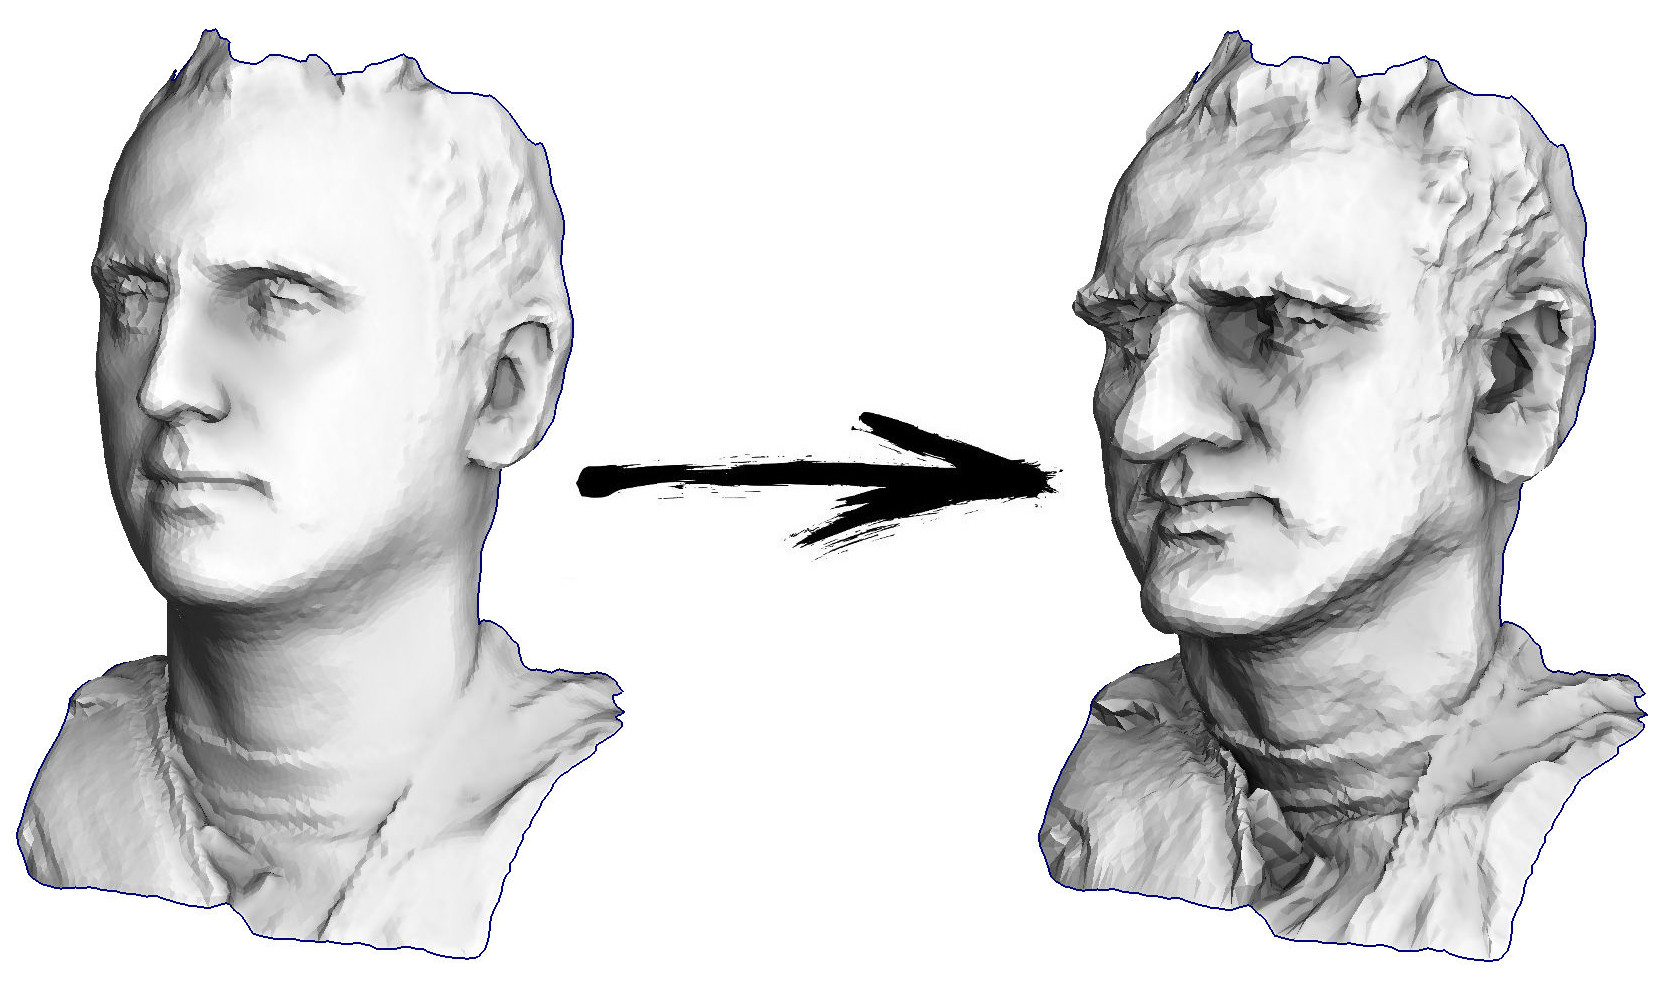
\includegraphics[width=.8\linewidth]{caricature.jpg}
	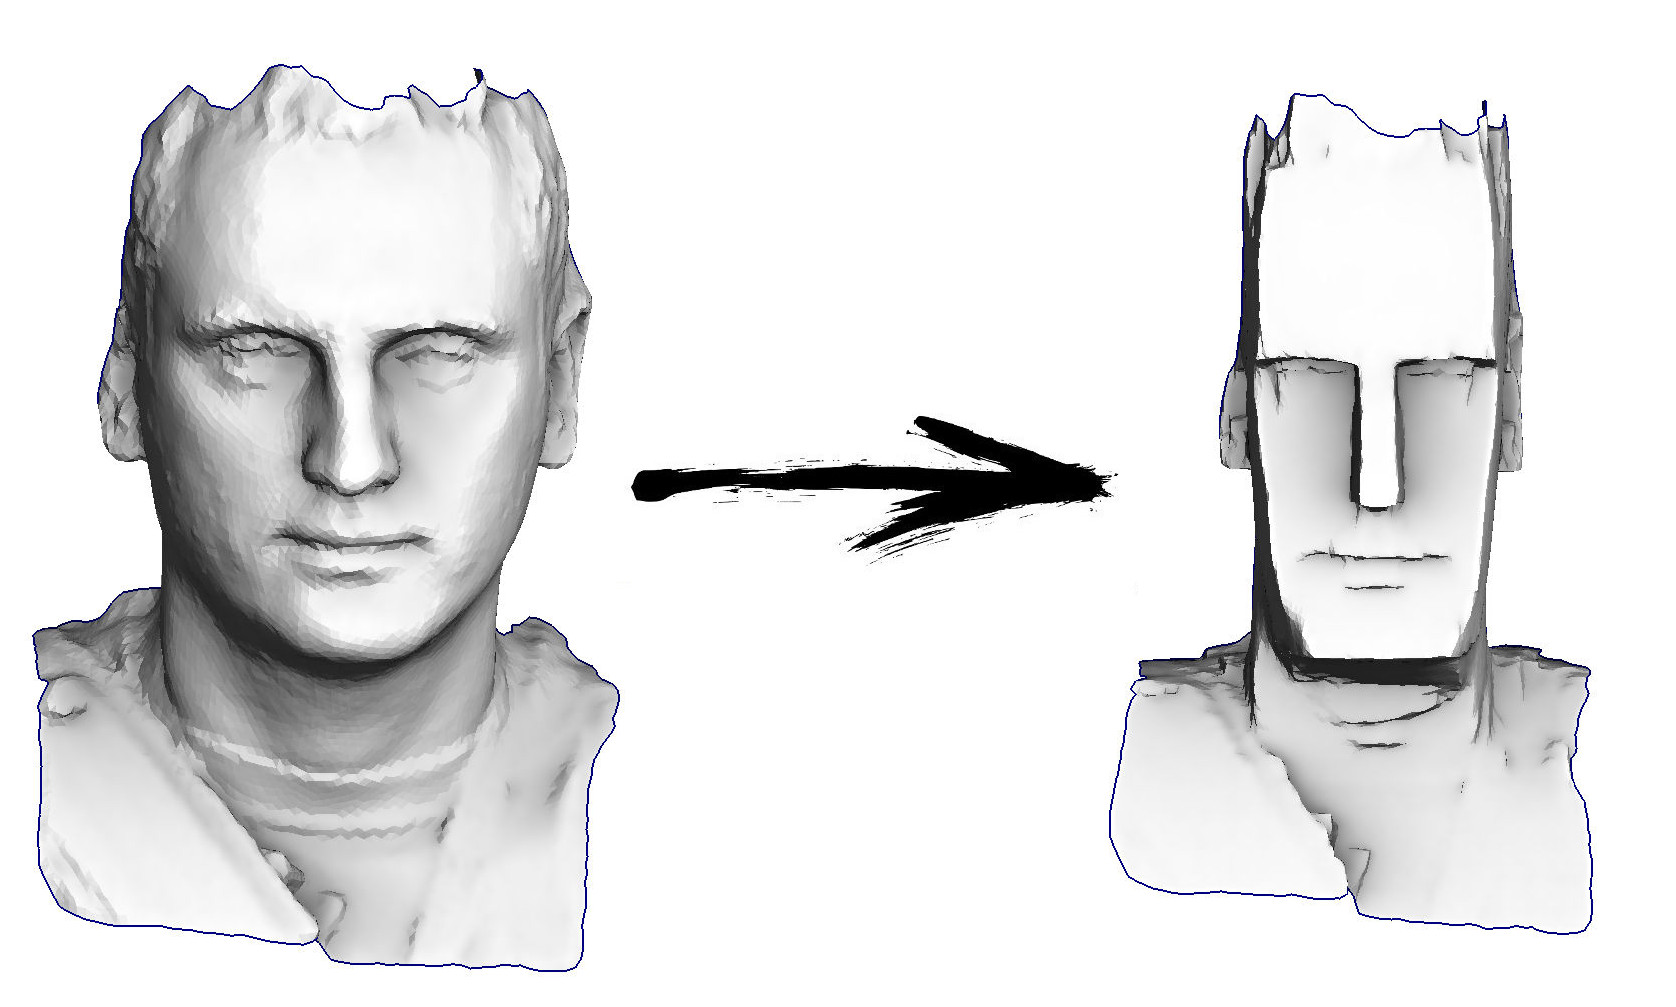
\includegraphics[width=.8\linewidth]{cubify.jpg}
	\caption{.}
	\label{fig:????}
\end{figure}


\begin{figure}[ht]
	\centering
    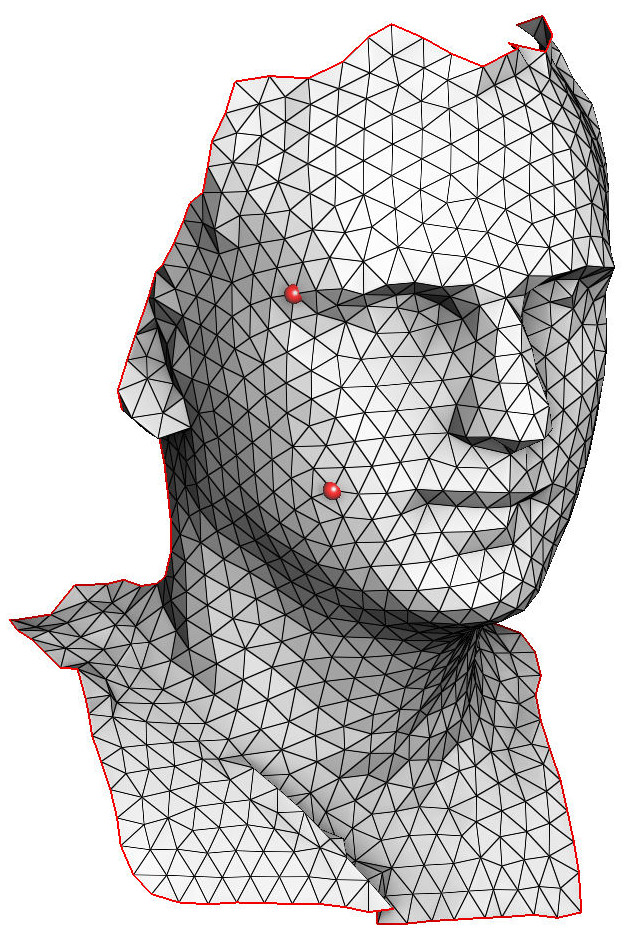
\includegraphics[width=.2\linewidth]{lscm-head-mesh.jpg}
    \quad
    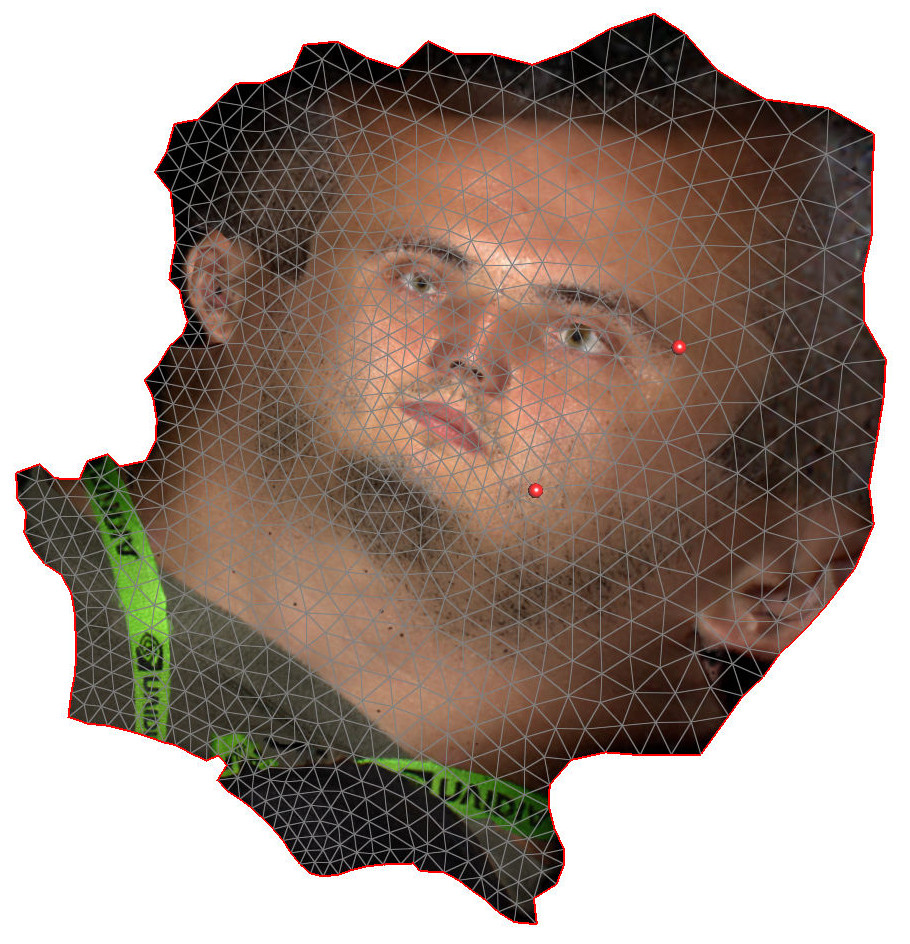
\includegraphics[width=.3\linewidth]{lscm-head-uv.jpg}
    \quad
    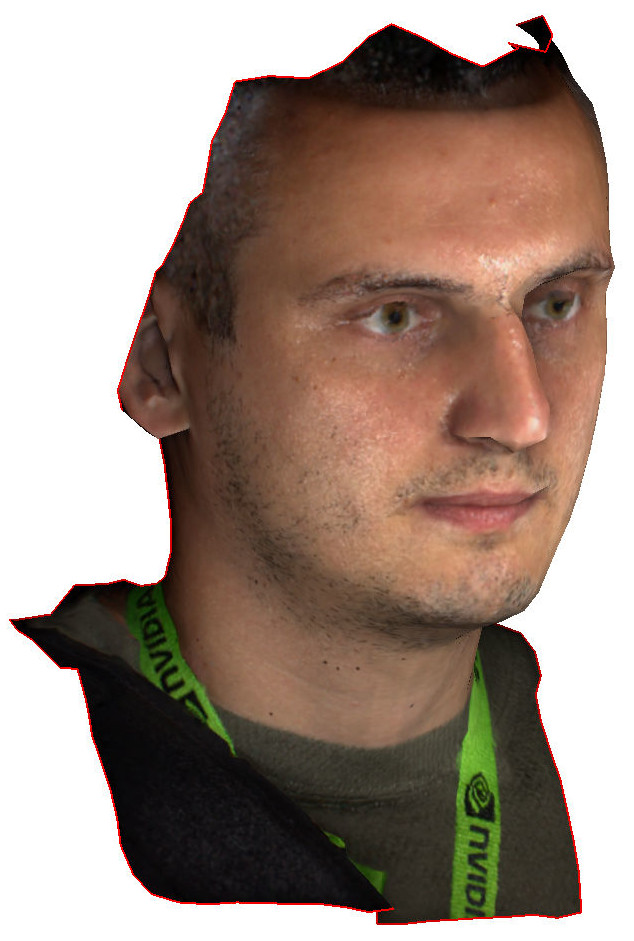
\includegraphics[width=.2\linewidth]{lscm-head-textured.jpg}
	\caption{Least squares conformal mapping. \textbf{Left:} input mesh; \textbf{middle:} unfolded mesh textured by an artist; \textbf{right:} final textured surface. Two pinned vertices are shown in red.}
	\label{fig:????}
\end{figure}


\chapter{From least squares to neural networks}
\section{Logistic regression}
Two possible classes encoded as $y \in \{0,1\}$ and assume
$$
p(y=1|x,w) = \frac{1}{1+e^{-w^\top x}},
$$
where $w$ is a $(m+1)$-parameter vector and the last element of $x$ is the constant 1.

Follows that
$$
p(y=0|x,w) = 1-P(y=1|x,w) = \frac{1}{1+e^{w^\top x}}
$$

Given $n$ independently distributed data points $x_i$ with corresponding labels $y_i$, we can write the log-likelihood as
$$
\log \mathcal{L}(w) = \log \prod_{i=1}^n p_i(w)^{y_i}  (1-p_i(w))^{1-y_i} = \sum_{i=1}^n \left(y_i w^\top x_i - \log\left(1+e^{w^\top x}\right)\right),
$$
where $p_i(w):=p(y_i=1|x_i, w)$.

To maximize $\log\mathcal L$, we set its derivatives to 0 and obtain
$$
\frac{\partial\log\mathcal L}{\partial w}(w) = \sum_{i=1}^n x_i(y_i-p_i(w)) = 0,
$$
so we have $m+1$ non-linear equations in $w$. 
We can rewrite the system as
\begin{equation}
\frac{\partial\log\mathcal L}{\partial w}(w) = X^\top (y-p) = 0,
\label{eq:logistic}
\end{equation}
where $X$ is the $n\times (m+1)$ matrix whose rows are $x_i$, $y:=\begin{bmatrix}y_1 & \dots & y_n\end{bmatrix}^\top$ and $p:=\begin{bmatrix}p_1(w) & \dots & p_n(w)\end{bmatrix}^\top$.

We can solve the system~\eqref{eq:logistic} iteratively using Newton-Raphson steps:
\begin{equation}
w^{(k+1)} = w^{(k)} - \left(\frac{\partial^2 \log \mathcal L}{\partial w \partial w^\top}\left(w^{(k)}\right)\right)^{-1}\frac{\partial \log \mathcal L}{\partial w}\left(w^{(k)}\right)
\label{eq:newton1}
\end{equation}
Let $V$ be $n\times n$ diagonal matrix with $V_{i,i} = p_i(w)(1-p_i(w))$, it is straightforward to verify that the Hessian matrix has the following expression:
$$
\frac{\partial^2 \log \mathcal L}{\partial w \partial w^\top}\left(w\right) = -X^\top V X.
$$
Then~\eqref{eq:newton1} becomes:
\begin{equation}
\label{eq:newton2}
\begin{split}
w^{(k+1)} &= w^{(k)} + \left(X^\top V^{(k)} X\right)^{-1} X^\top (y - p^{(k)}) \\
          &= \left(X^\top V^{(k)} X\right)^{-1} X^\top V^{(k)} \left(X w^{(k)} + {V^{(k)}}^{-1} (y - p^{(k)})\right) \\
          &= \left(X^\top V^{(k)} X\right)^{-1} X^\top V^{(k)} z^{(k)},
\end{split}
\end{equation}
where $z^{(k)}:=Xw^{(k)} + {V^{(k)}}^{-1} (y - p^{(k)})$ and where $V^{(k)}$ and $p^{(k)}$ are $V$ and $p$, respectively, evaluated at $w^{(k)}$.

Note that $w^{(k+1)}$ as given by~\eqref{eq:newton2} also satisfies
$$
w^{(k+1)} = \argmin\limits_w \left(z^{(k)}-Xw\right)^\top V^{(k)} \left(z^{(k)}-Xw\right),
$$
a weighted least-squares problem, and hense iterating~\eqref{eq:newton2} is often called iteratively reweighted least squares.
It is easy to see that the Hessian matrix $X^\top V X$ is positive definite (it follows from the fact that $V>0$), and thus is a convex optimization problem.

Note that convergence fails if the two classes are linearly separable. In that case we can handle this via a regularization.



\end{document}

